\graphicspath{{R250410/Figs/}}

\section*{Permanent GNSS stations}
 % ------------------------------------------------------------------------------
\begin{frame}
  \frametitle{Permanent GNSS stations}
  \framesubtitle{}
  \label{}
  \vskip-.5cm
  \begin{columns}[T]
    \begin{column}{.4\textwidth}
      \begin{center}
        \textbf{Network GREECE}\\
        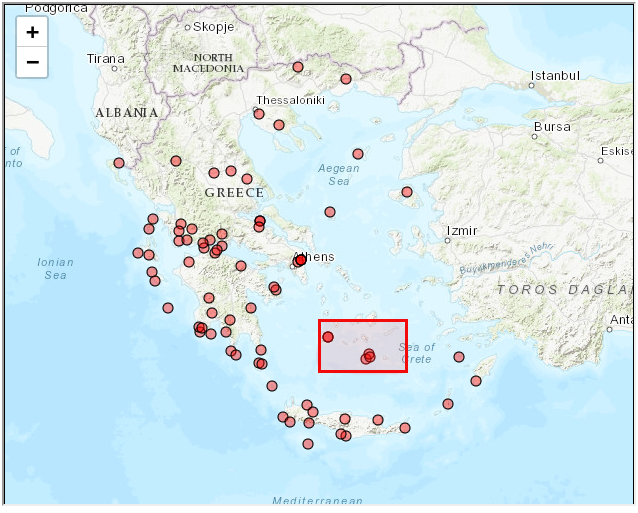
\includegraphics[width=.97\textwidth]{gnsssta_gre.png}
      \end{center}        
    \end{column}
    \begin{column}{.6\textwidth}
      \begin{center}
        \textbf{Network SANTORINI}\\
        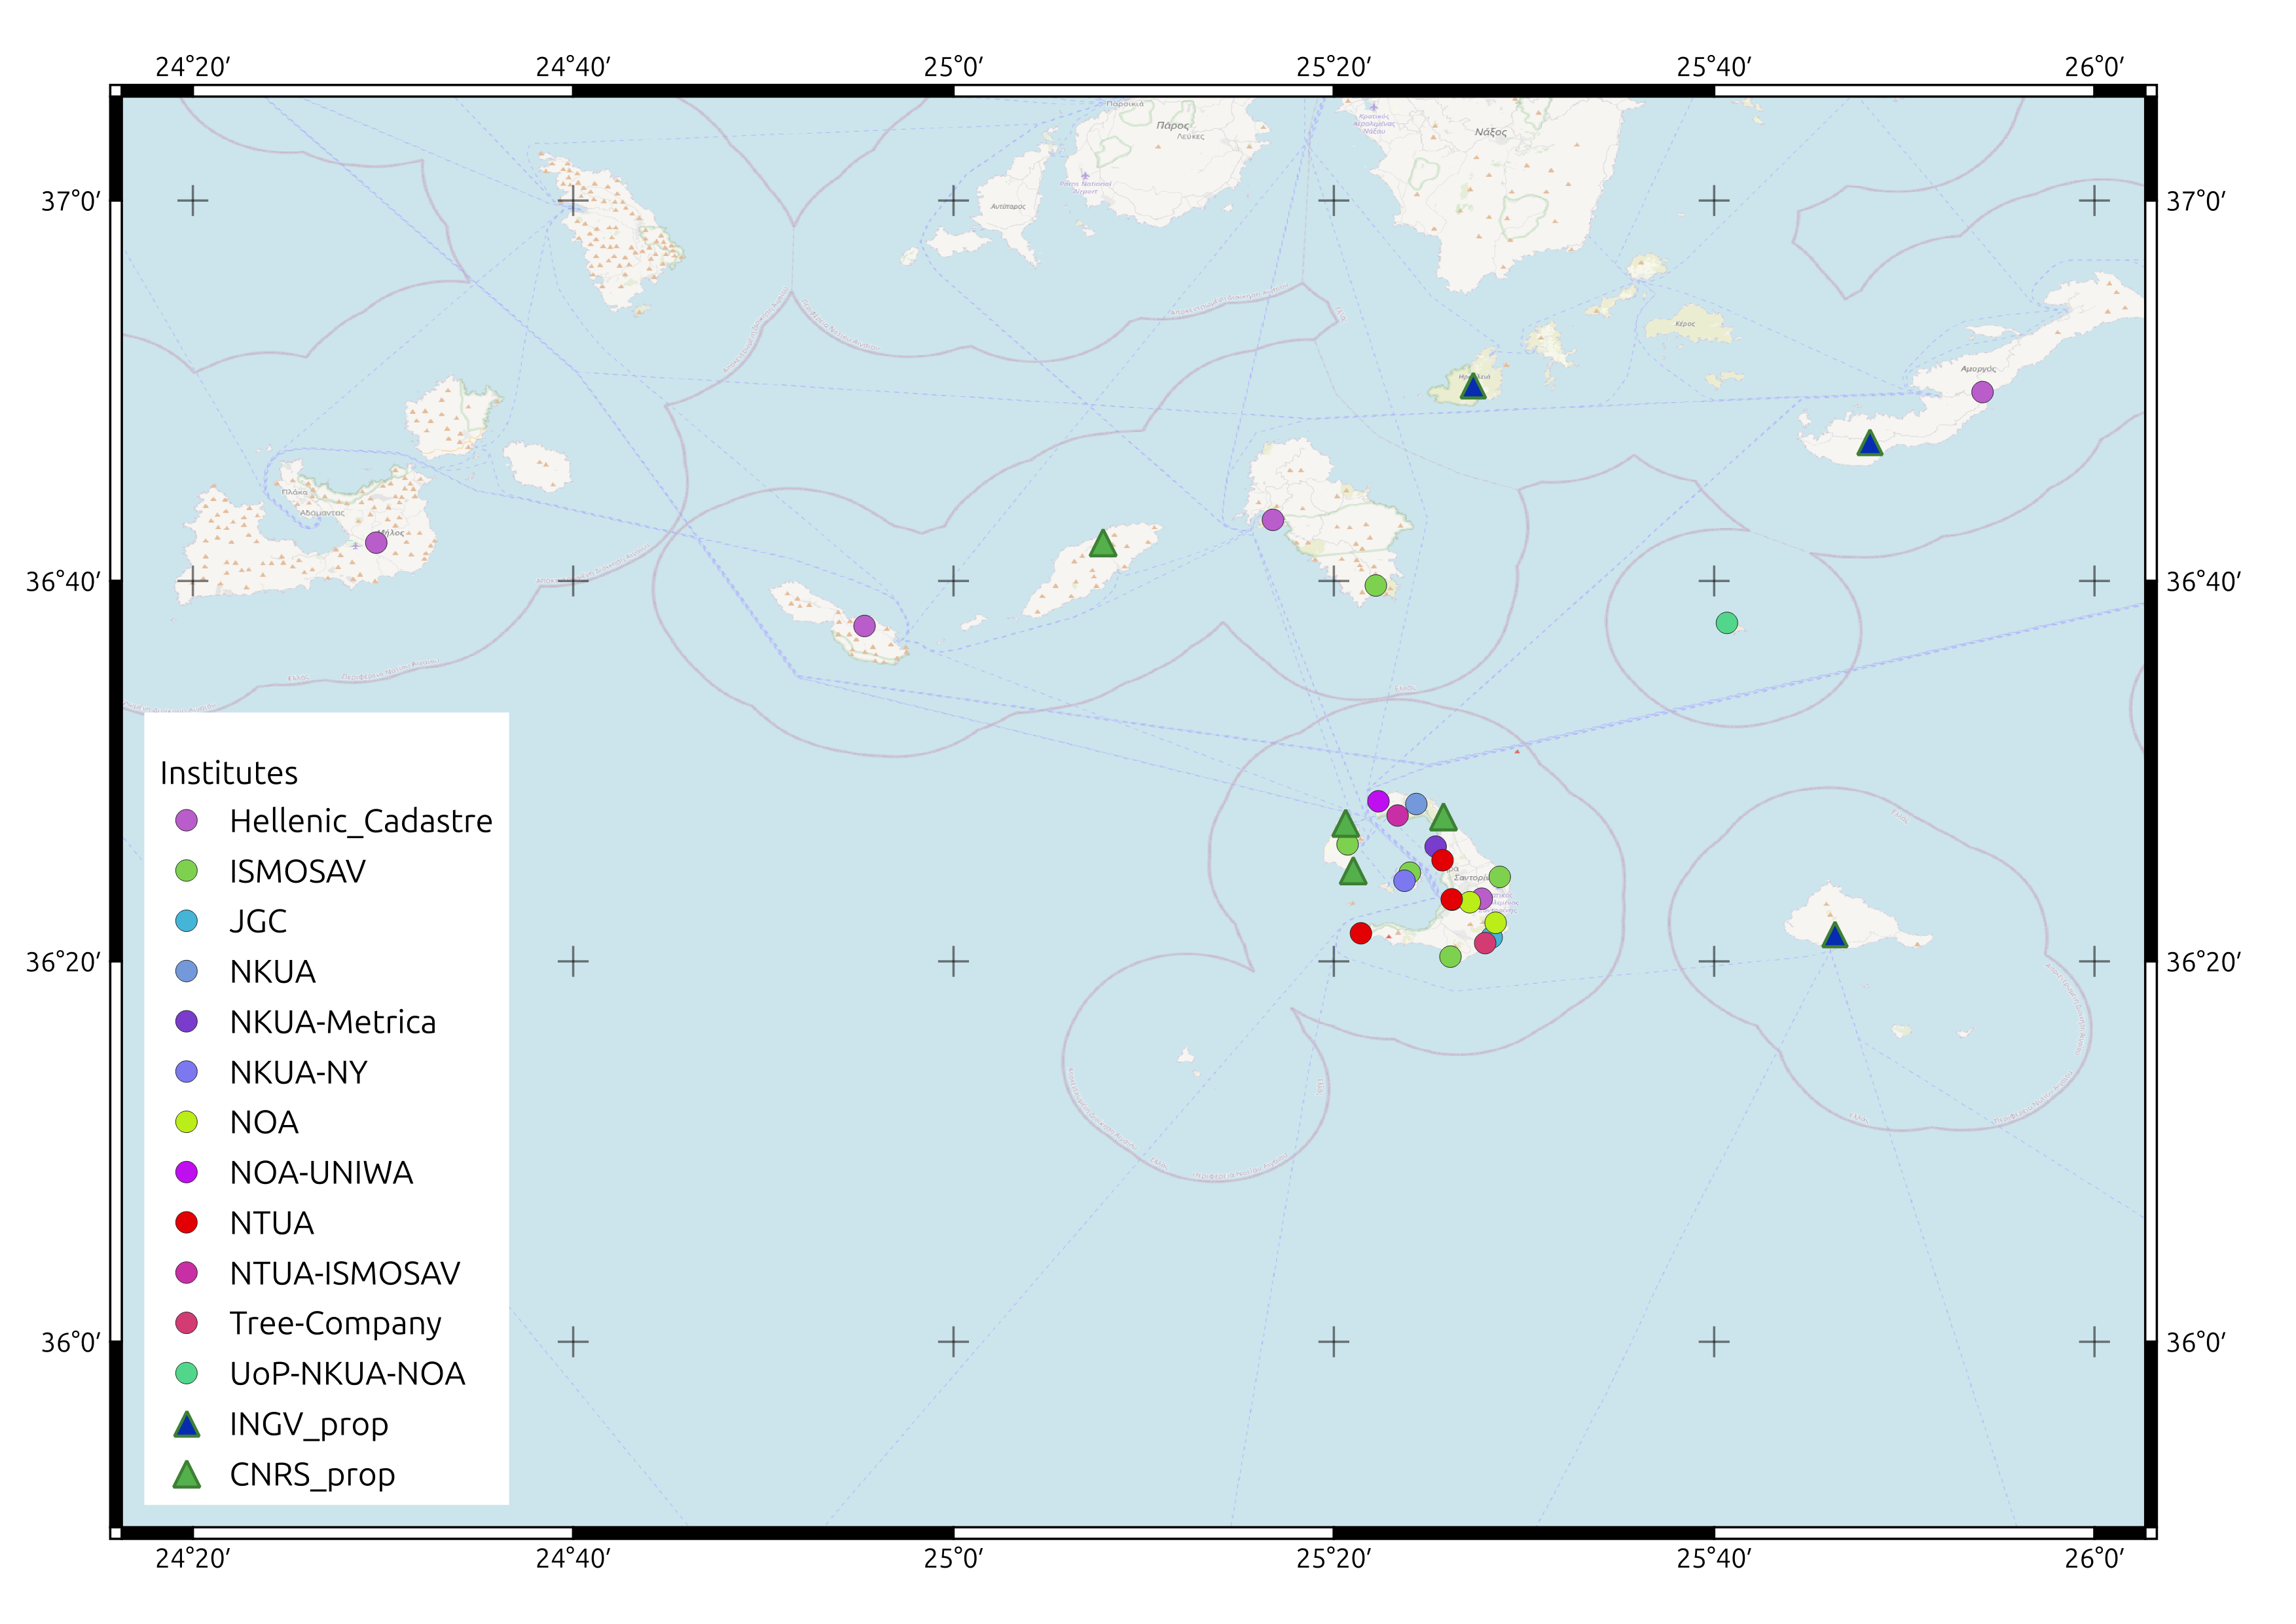
\includegraphics[width=.97\textwidth]{ccyclades_gnss.png}
      \end{center}
    \end{column}
  \end{columns}
\end{frame}
\note{}

 % ------------------------------------------------------------------------------
\begin{frame}
  \frametitle{Station maintenance}
  \framesubtitle{}
  \label{}
  \vskip-1cm
  \begin{columns}[T]
    \begin{column}{.25\textwidth}
      \begin{center}
      {\scriptsize SNTR 12653M001}
        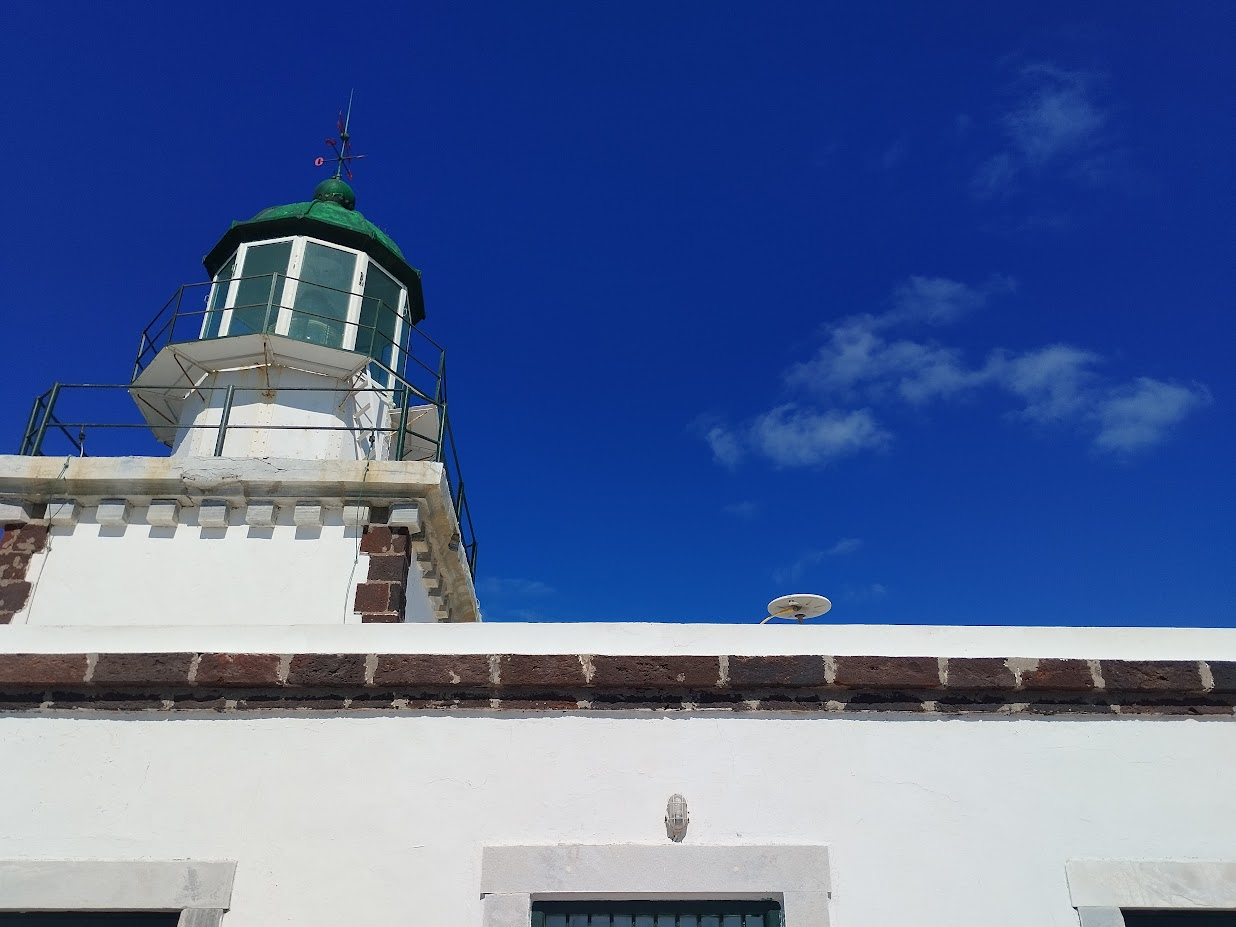
\includegraphics[width=.97\textwidth]{SNTR_01.jpg}
      \end{center}  
    \end{column}
    \begin{column}{.25\textwidth}
      \begin{center}
       {\scriptsize WNRY 12687M001}
        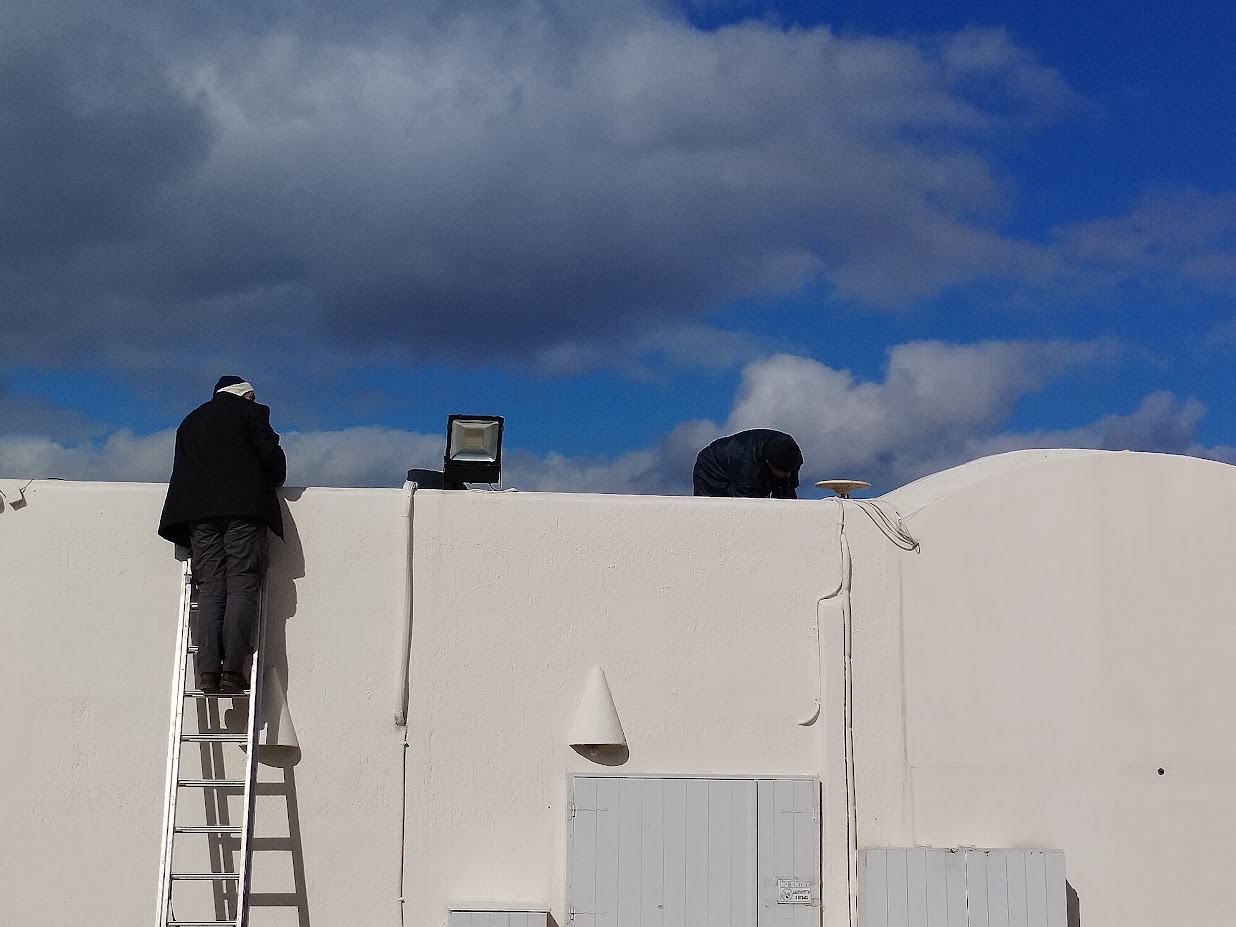
\includegraphics[width=.97\textwidth]{wnry_01.jpg}
      \end{center}       
    \end{column}
  \begin{column}{.25\textwidth}
      \begin{center}
       {\scriptsize NOMI}
        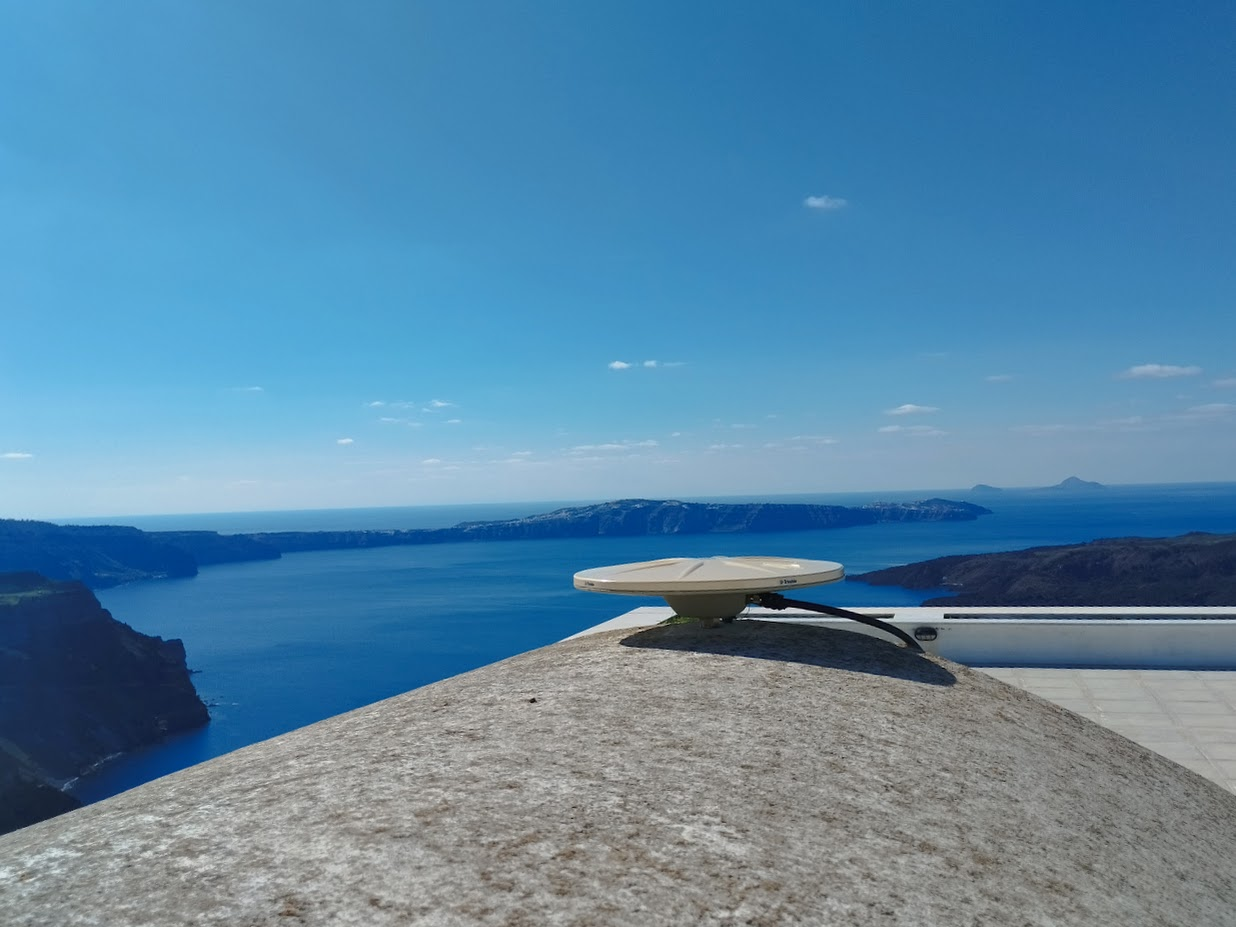
\includegraphics[width=.97\textwidth]{NOMI_01.jpg}
      \end{center}  
    \end{column}
    \begin{column}{.25\textwidth}
      \begin{center}
       {\scriptsize Campaign}
        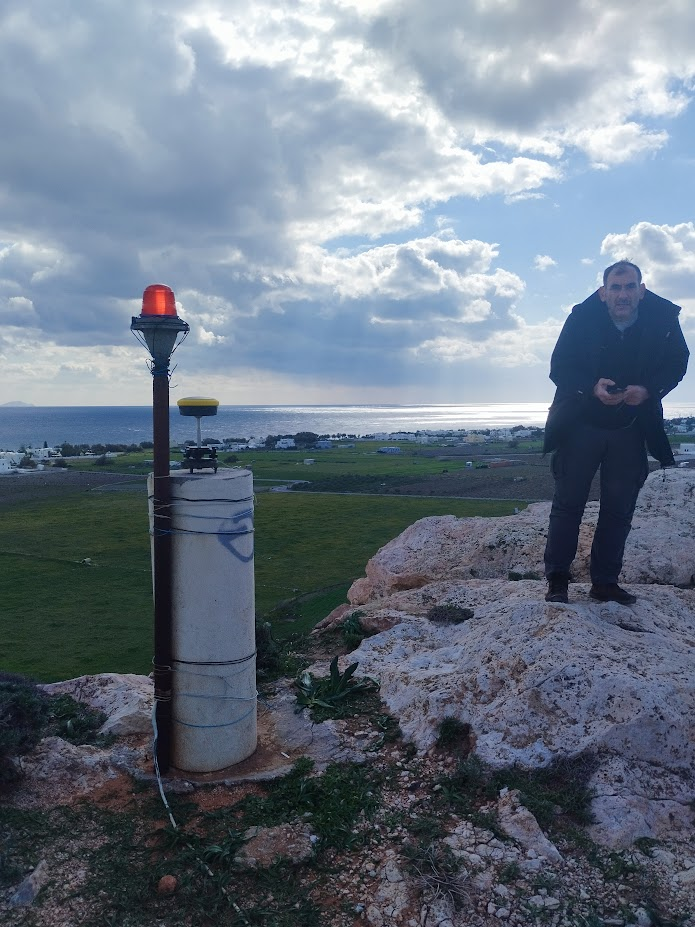
\includegraphics[width=.7\textwidth]{sn_camp.jpg}
      \end{center}       
    \end{column}
  \end{columns}  
  ~\\[1em]
\begin{scriptsize}
- Daily RINEX availability: \url{http://dionysos.survey.ntua.gr/dsoportal/\_datacenter/httpdata.html}\\
- Station ΝΟΜΙ is available in colaboration with University of Patras and EarthScope.
\end{scriptsize}

\end{frame}
\note{}


\section*{Ανάλυση δεδομένων}

 % ------------------------------------------------------------------------------
\begin{frame}
  \frametitle{GNSS data analysis at DSO}
  \framesubtitle{}
  \label{}
  \begin{columns}[T]
    \begin{column}{.5\textwidth}
    \textbf{GNSS data analysis}
      \begin{itemize}\setlength\itemsep{1em}
         \item Bernese v5.2 / v5.4 \citep{Bernese}
         \item PRIDE-PPPAR \citep{PRIDE}
         \item GipsyX \citep{GipsyX}
       \end{itemize} 
    \textbf{Time series analysis}
    \begin{itemize}\setlength\itemsep{1em}
      \item Hector v2.1 \citep{Bos2012}
      \item Python/C++ routines
    \end{itemize}
    \end{column}
    \begin{column}{.5\textwidth}
      \textbf{Solutions}
      \begin{itemize}\setlength\itemsep{1em}
        \item Daily solution
          \begin{itemize}\setlength\itemsep{1em}
            \item Rapid solution - 1 day after
            \item Final solution - 12 days after
          \end{itemize}
        \item High-rate analysis (>1Hz)
          \begin{itemize}\setlength\itemsep{1em}
            \item data from network HEPOS - 1Hz
          \end{itemize}
      \end{itemize}
    \end{column}
  \end{columns}
  \begin{columns}[T]
    \begin{column}{.1\textwidth}
      \begin{center}
        \includegraphics[width=.7\textwidth]{logo_Bernese.png}
      \end{center}
    \end{column}
    \begin{column}{.2\textwidth}
      \begin{center}
        
\includegraphics[width=.97\textwidth]{logo_PRIDE.png}
      \end{center}      
    \end{column}
    \begin{column}{.2\textwidth}
      \begin{center}
        
\includegraphics[width=.8\textwidth]{logo_gipsyX.png}
      \end{center}      
    \end{column}
    \begin{column}{.5\textwidth}
      \begin{center}

      \end{center}      
    \end{column}    
    
  \end{columns}
\end{frame}
\note{}

 % ------------------------------------------------------------------------------
\begin{frame}
  \frametitle{Automated processing scheme}
  \framesubtitle{}
  \label{}
\vskip-.5cm
\begin{columns}[T]
  \begin{column}{.55\textwidth}
 \begin{center}
    \begin{tikzpicture}[ every annotation/.style = {draw,
                      fill = white, font = \large}]

   \path[mindmap,concept color=black!70,text=white,
     every node/.style={concept,circular drop shadow, scale=.42},
     root/.style = {concept color=black!30!red!50,
font=\normalsize\bfseries,text width=5em},
     level 1 concept/.append style={
       font=\normalsize\bfseries, sibling angle=70,text width=7.7em,
       level distance=20mm,inner sep=0pt},
     level 2 concept/.append style={font=\bfseries,level distance=15mm},
   ]

   node[root] {Bernese GNSS Software v5.2} [clockwise from=0]
     child[concept color=red!50] {
       node {pyBern Module} [clockwise from=140]
       child  [color=black!80] { node {github repo} }
       child  { node {handle PCF, BPE, flow-control} }
       child  { node {parsers\\formaters} }
       child  { node {pre-processing \& editing} }
       child  [level distance=13mm] { node {data/product downloading} }
     }
     child[concept color=blue!60] {
       node[concept] {MySQL Database} [clockwise from=-10]
       child { node[concept] {from/to .STA} }
       child { node[concept] {stations/ networks/ products} }
       child [level distance=17mm] { node[concept] {IGS log files} }
     }
     child[concept color=red!80] {
       node[concept] {Cron Jobs} [clockwise from=-40]
       child [level distance=13mm] { node[concept] {final ultra-rapid} }
       child { node[concept] {update ATX, PCV } }
       child { node[concept] {sync with AIUB} }
       child [level distance=12mm, sibling angle=70] { node[concept]
{sync with M3G} }
     }
     child[concept color=orange!60!black!30] {
       node[concept] { Analysis } [clockwise from=220]
       child { node[concept] {Time-Series} }
       child [text width=]{ node[concept] {StrainTool} }
     }
     child[concept color=green!70] {
       node[concept] { WebPage } [clockwise from=180]
       child [level distance=12mm, text width=] { node[concept] {d3.js
plots} }
     };
\end{tikzpicture}
\end{center}
  \end{column}
  \begin{column}{.45\textwidth}
    Standards:
  \begin{itemize}\setlength\itemsep{.1em}
    \item \texttt{SINEX} with required info/blocks,
    \item Reference frame \texttt{\textcolor{red}{IGS20}},
    \item \texttt{IERS} Conventions 2010,
    \item \texttt{IGS}/\texttt{CODE} products,
    \item ocean loading corrections (\texttt{\textcolor{red}{FES2014b}}),
    %\item atmospheric tidal loading corrections,
    \item $3^{\circ}$ elevation cut-off angle; elevation dependent weighting,
    \item \texttt{GMF} and/or \texttt{\textcolor{red}{VMF1}}; \texttt{Chen-Herring} gradient parameter,
    \item amiguities fixed (length-dependent algorithm),
    \item use \texttt{GLONASS} obs (when available)
    \item use \texttt{ATX} files  (\textcolor{red}{epn\_20.atx})
  \end{itemize}
  \end{column}
\end{columns}

\end{frame}
\note{}


 % ------------------------------------------------------------------------------
\begin{frame}
  \frametitle{Time series analysis}
  \framesubtitle{}
  \label{}
  \vskip-1cm
  \begin{columns}[T]
    \begin{column}{.25\textwidth}
      \begin{center}
      {\scriptsize 047A (Amorgos)}
        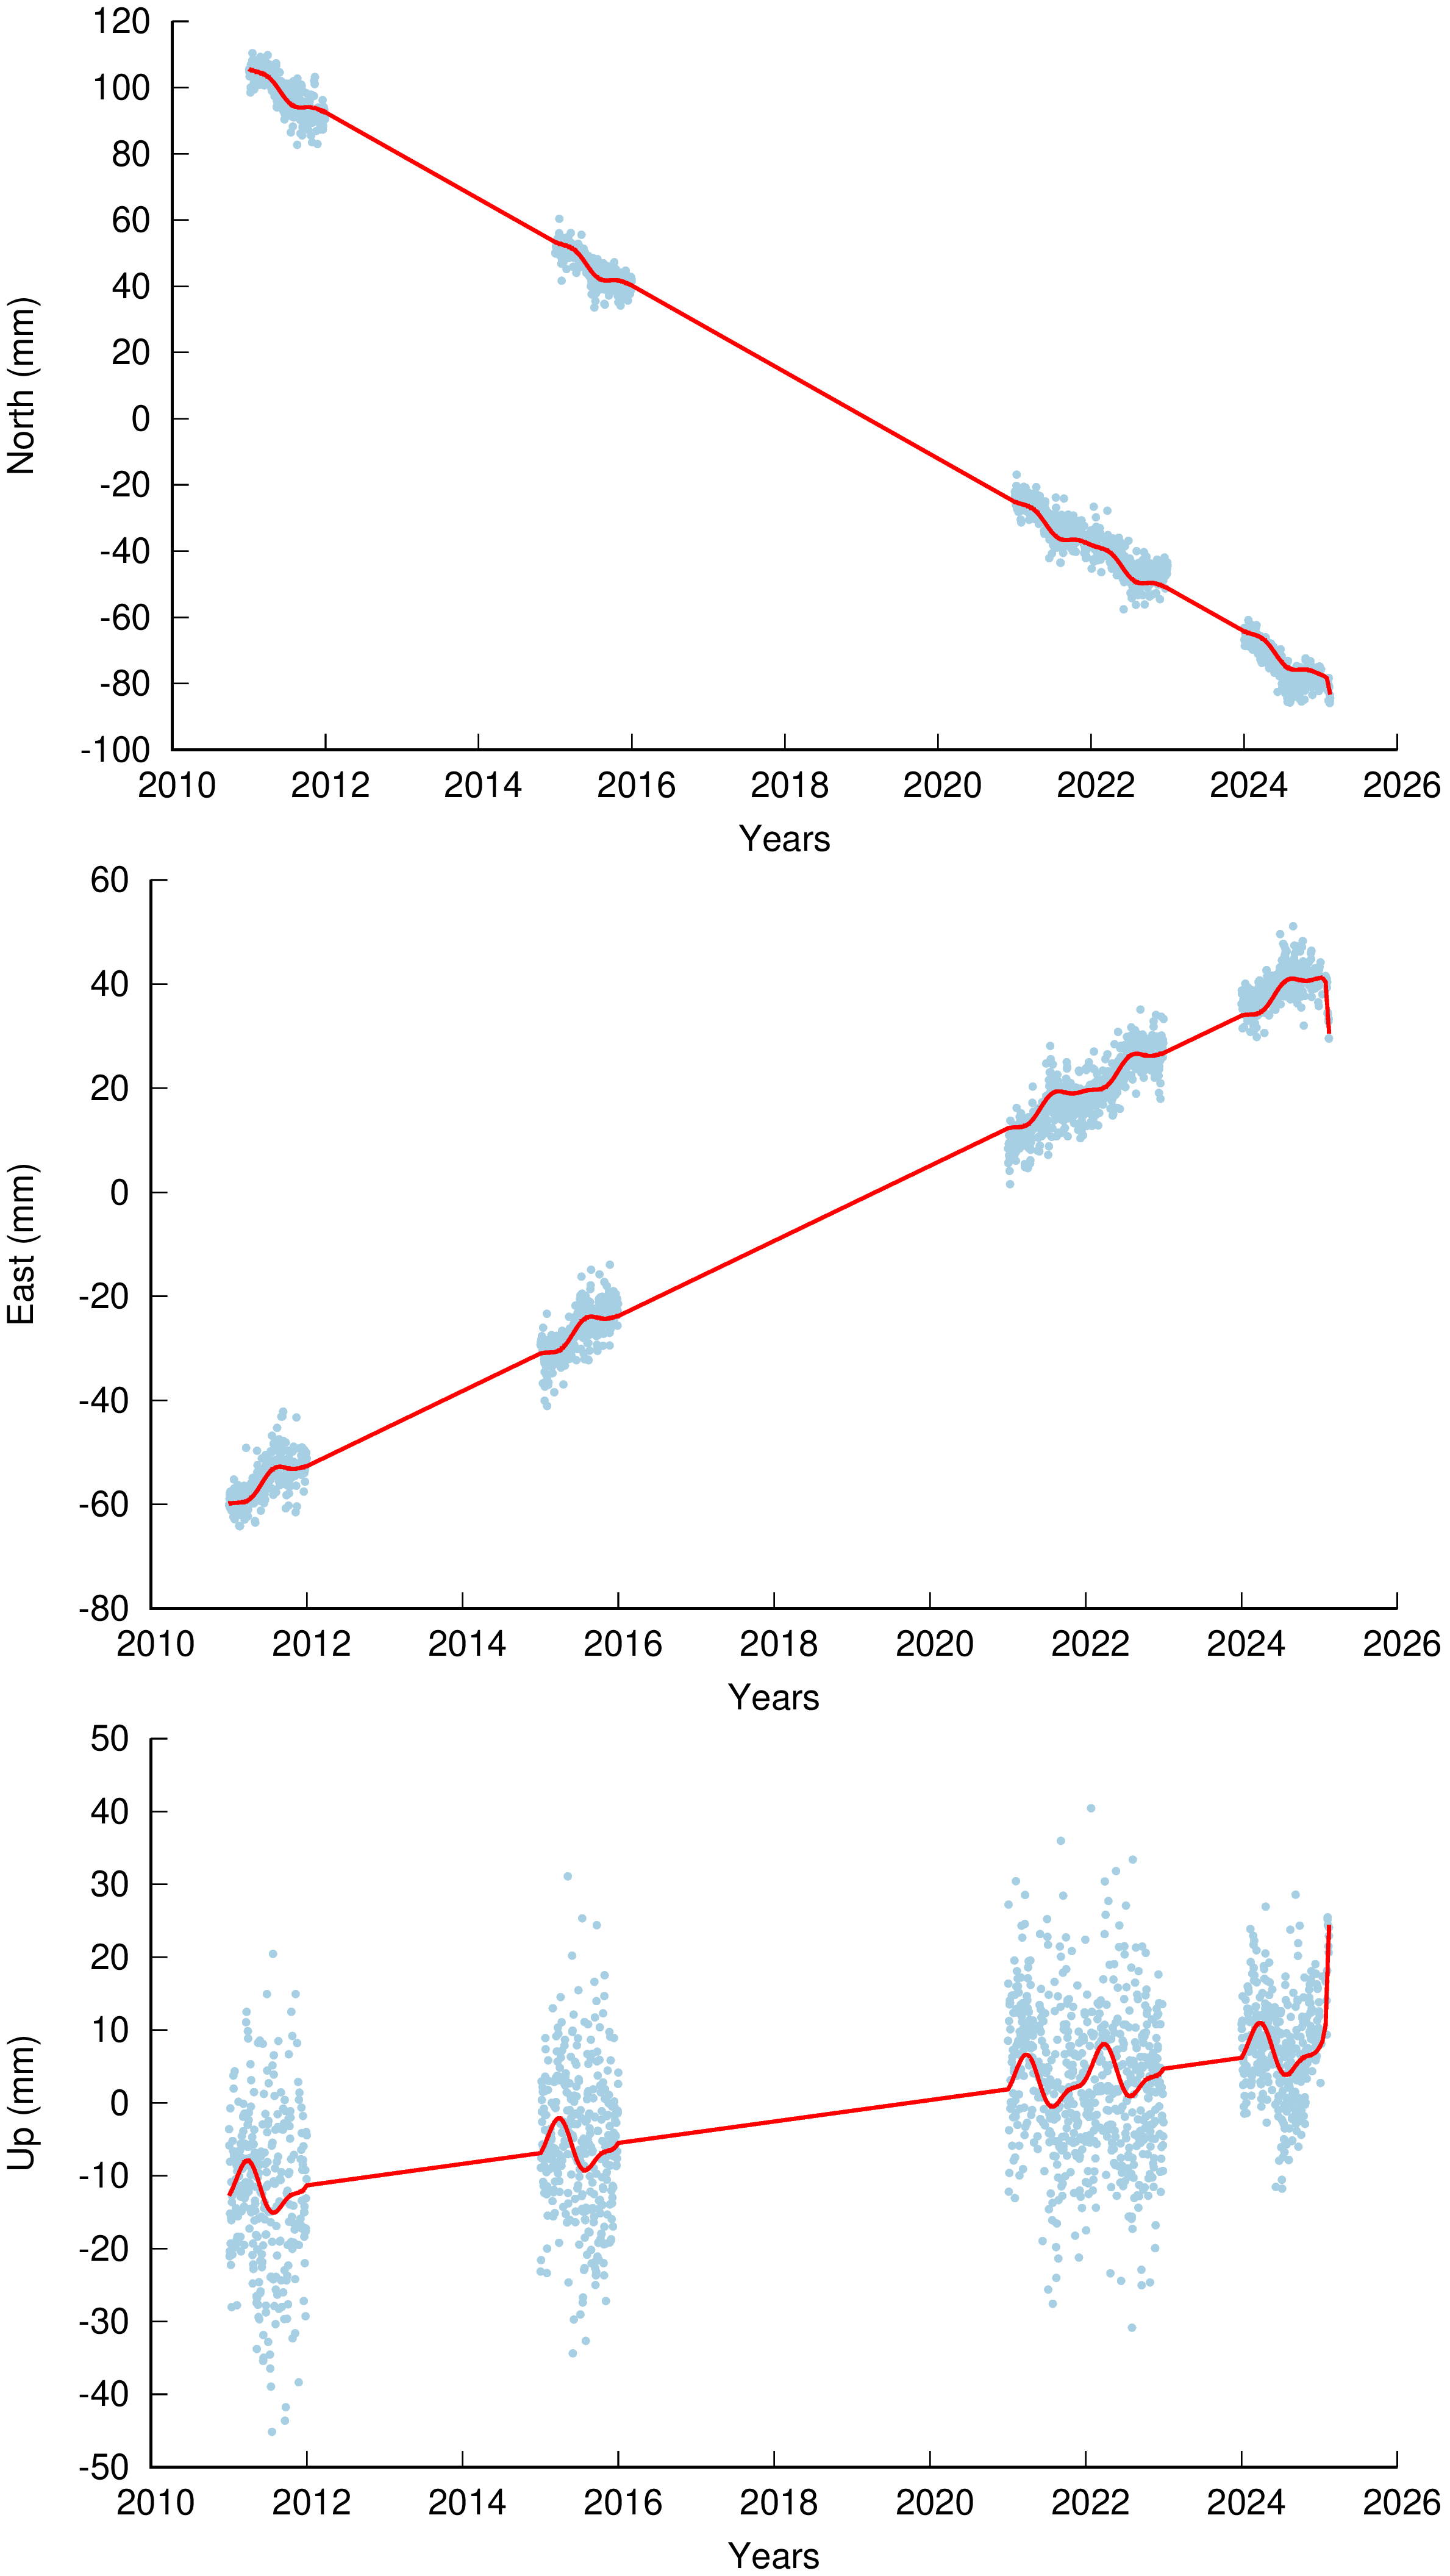
\includegraphics[width=.97\textwidth]{047a-mod.png}
      \end{center}  
    \end{column}
    \begin{column}{.25\textwidth}
      \begin{center}
       {\scriptsize 049A (Ios)}
        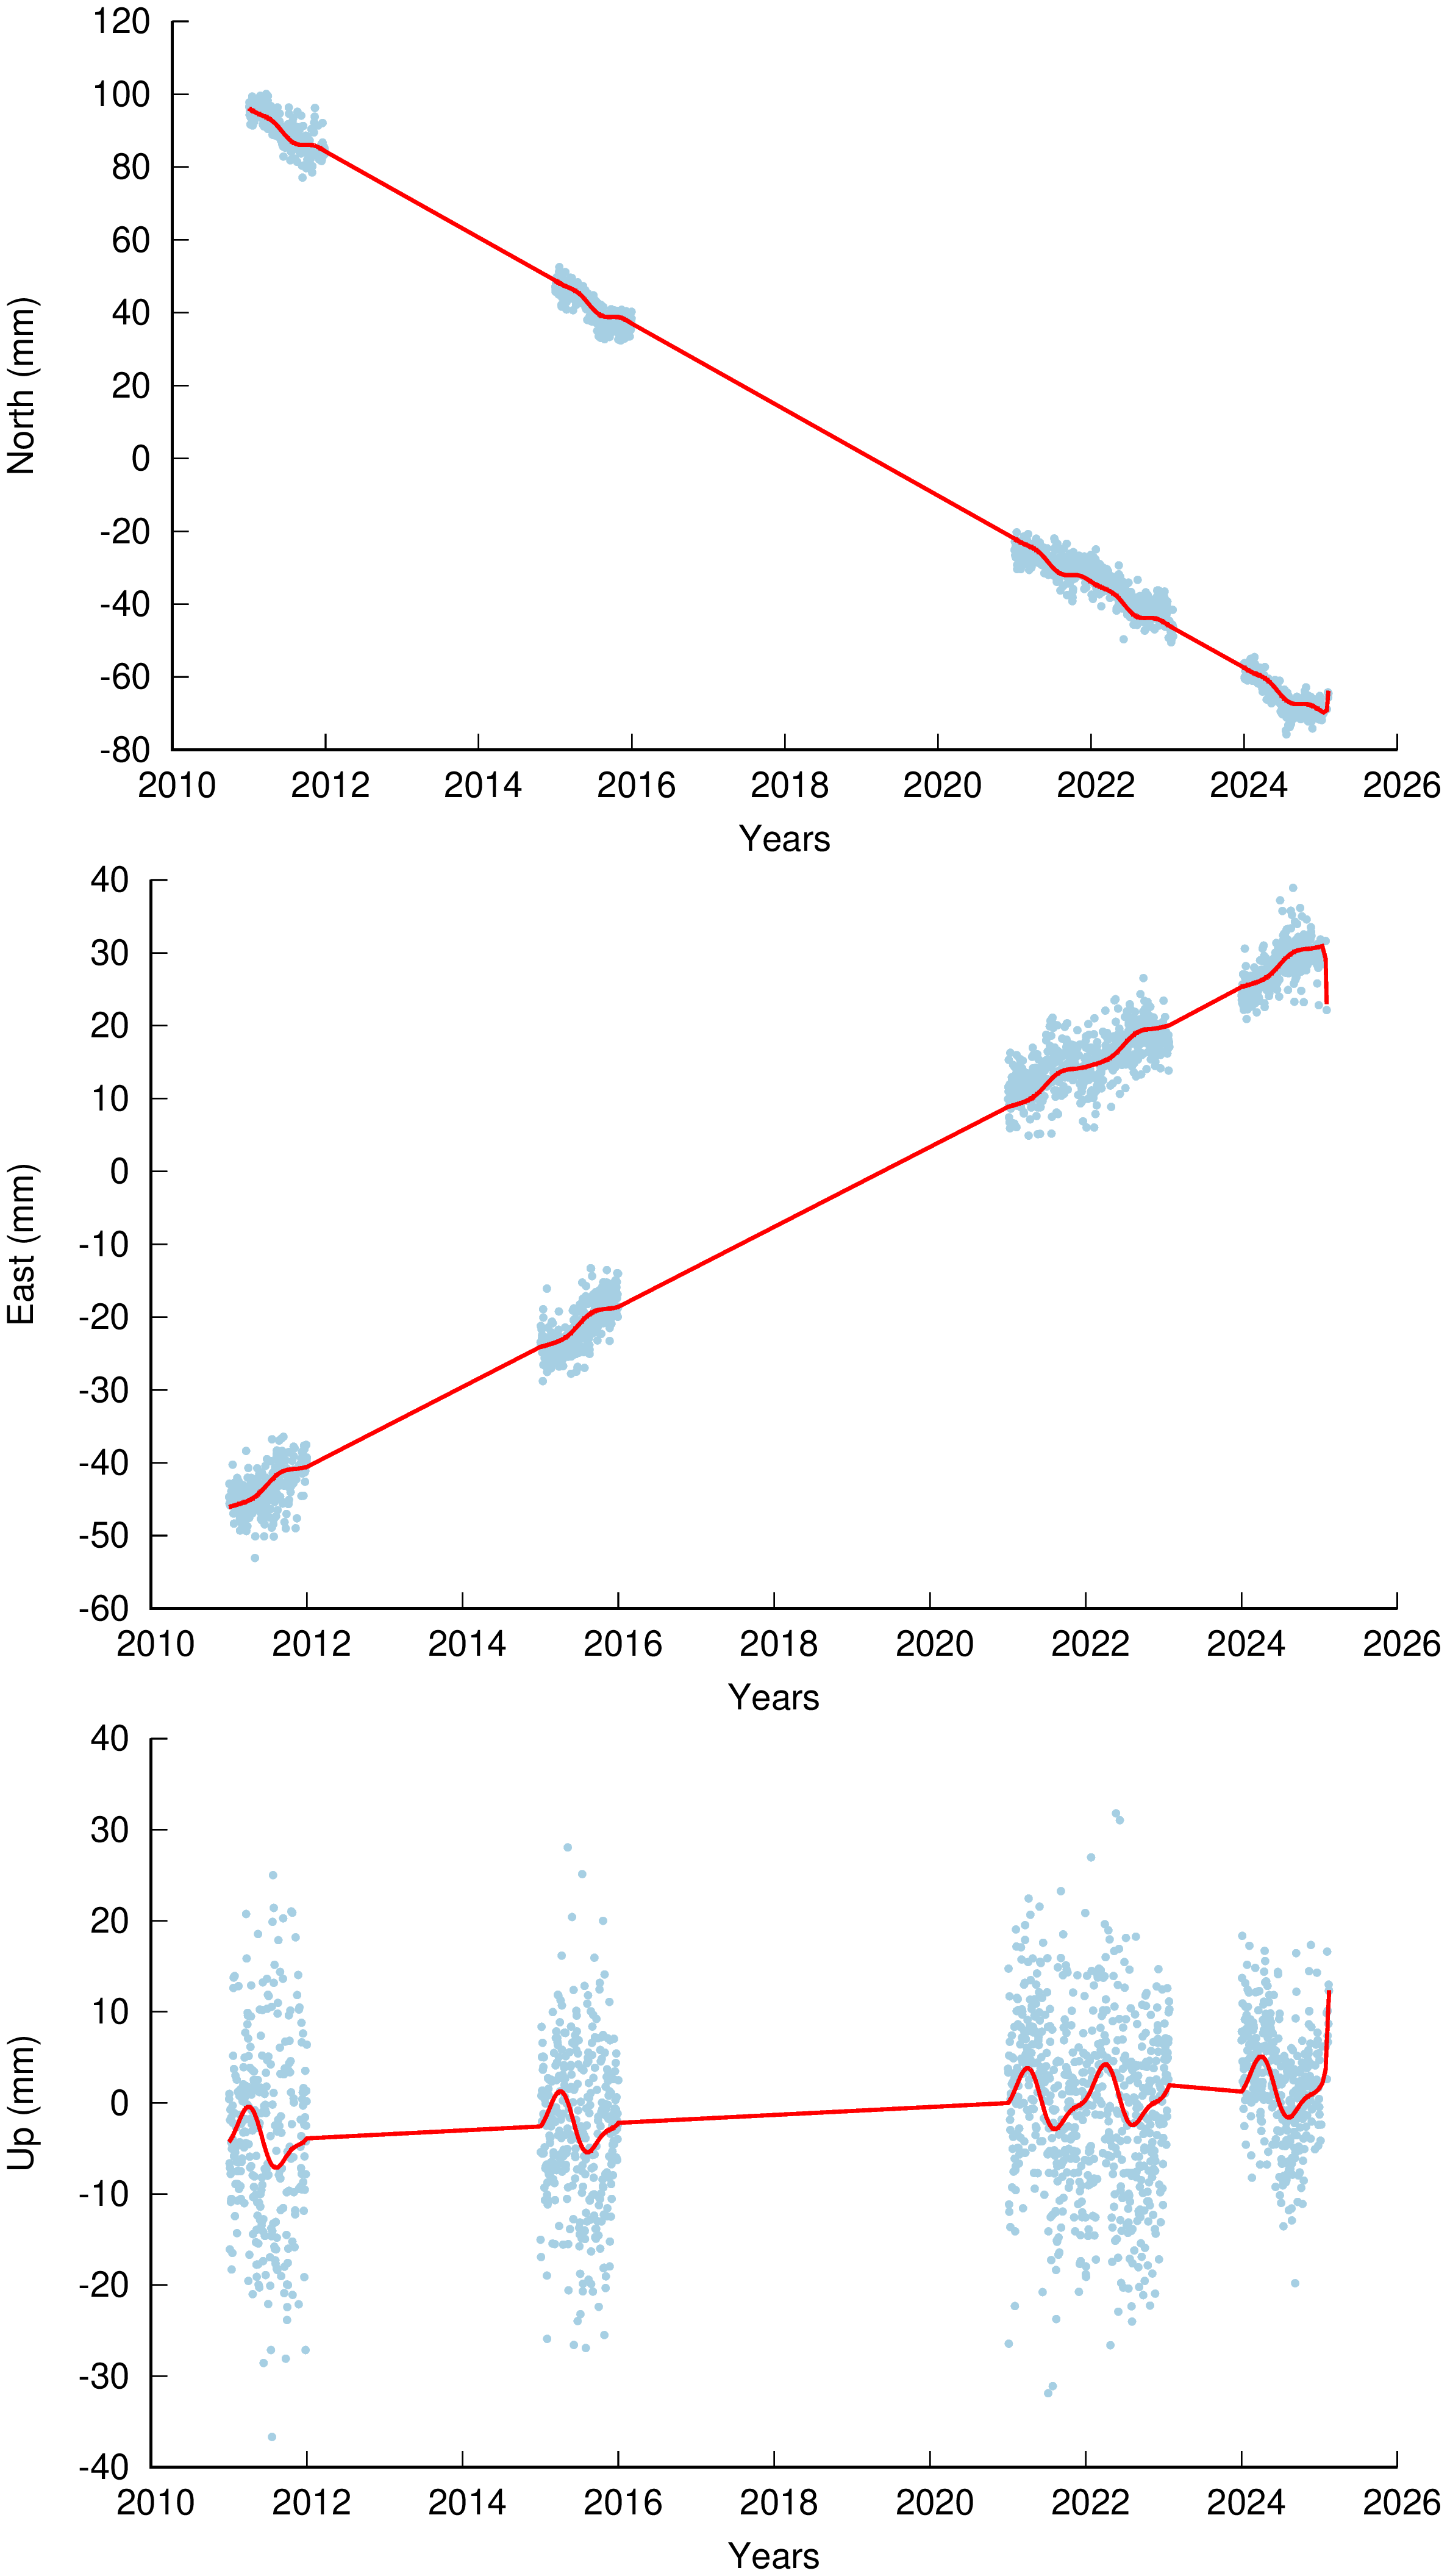
\includegraphics[width=.97\textwidth]{049a-mod.png}
      \end{center}       
    \end{column}
  \begin{column}{.25\textwidth}
      \begin{center}
       {\scriptsize 048A (Thira)}
        
\includegraphics[width=.97\textwidth]{048a-mod.png}
      \end{center}  
    \end{column}
    \begin{column}{.25\textwidth}
      \begin{center}
       {\scriptsize SNTR (Faros)}
        
\includegraphics[width=.97\textwidth]{sntr-mod.png}
      \end{center}       
    \end{column}
  \end{columns}  
  
\end{frame}
\note{}


 % ------------------------------------------------------------------------------
\begin{frame}
  \frametitle{Tectonic velocities [IGS20]}
  \framesubtitle{}
  \label{}
  \vskip-1cm
  \begin{columns}[T]
    \begin{column}{.5\textwidth}
      \begin{center}
        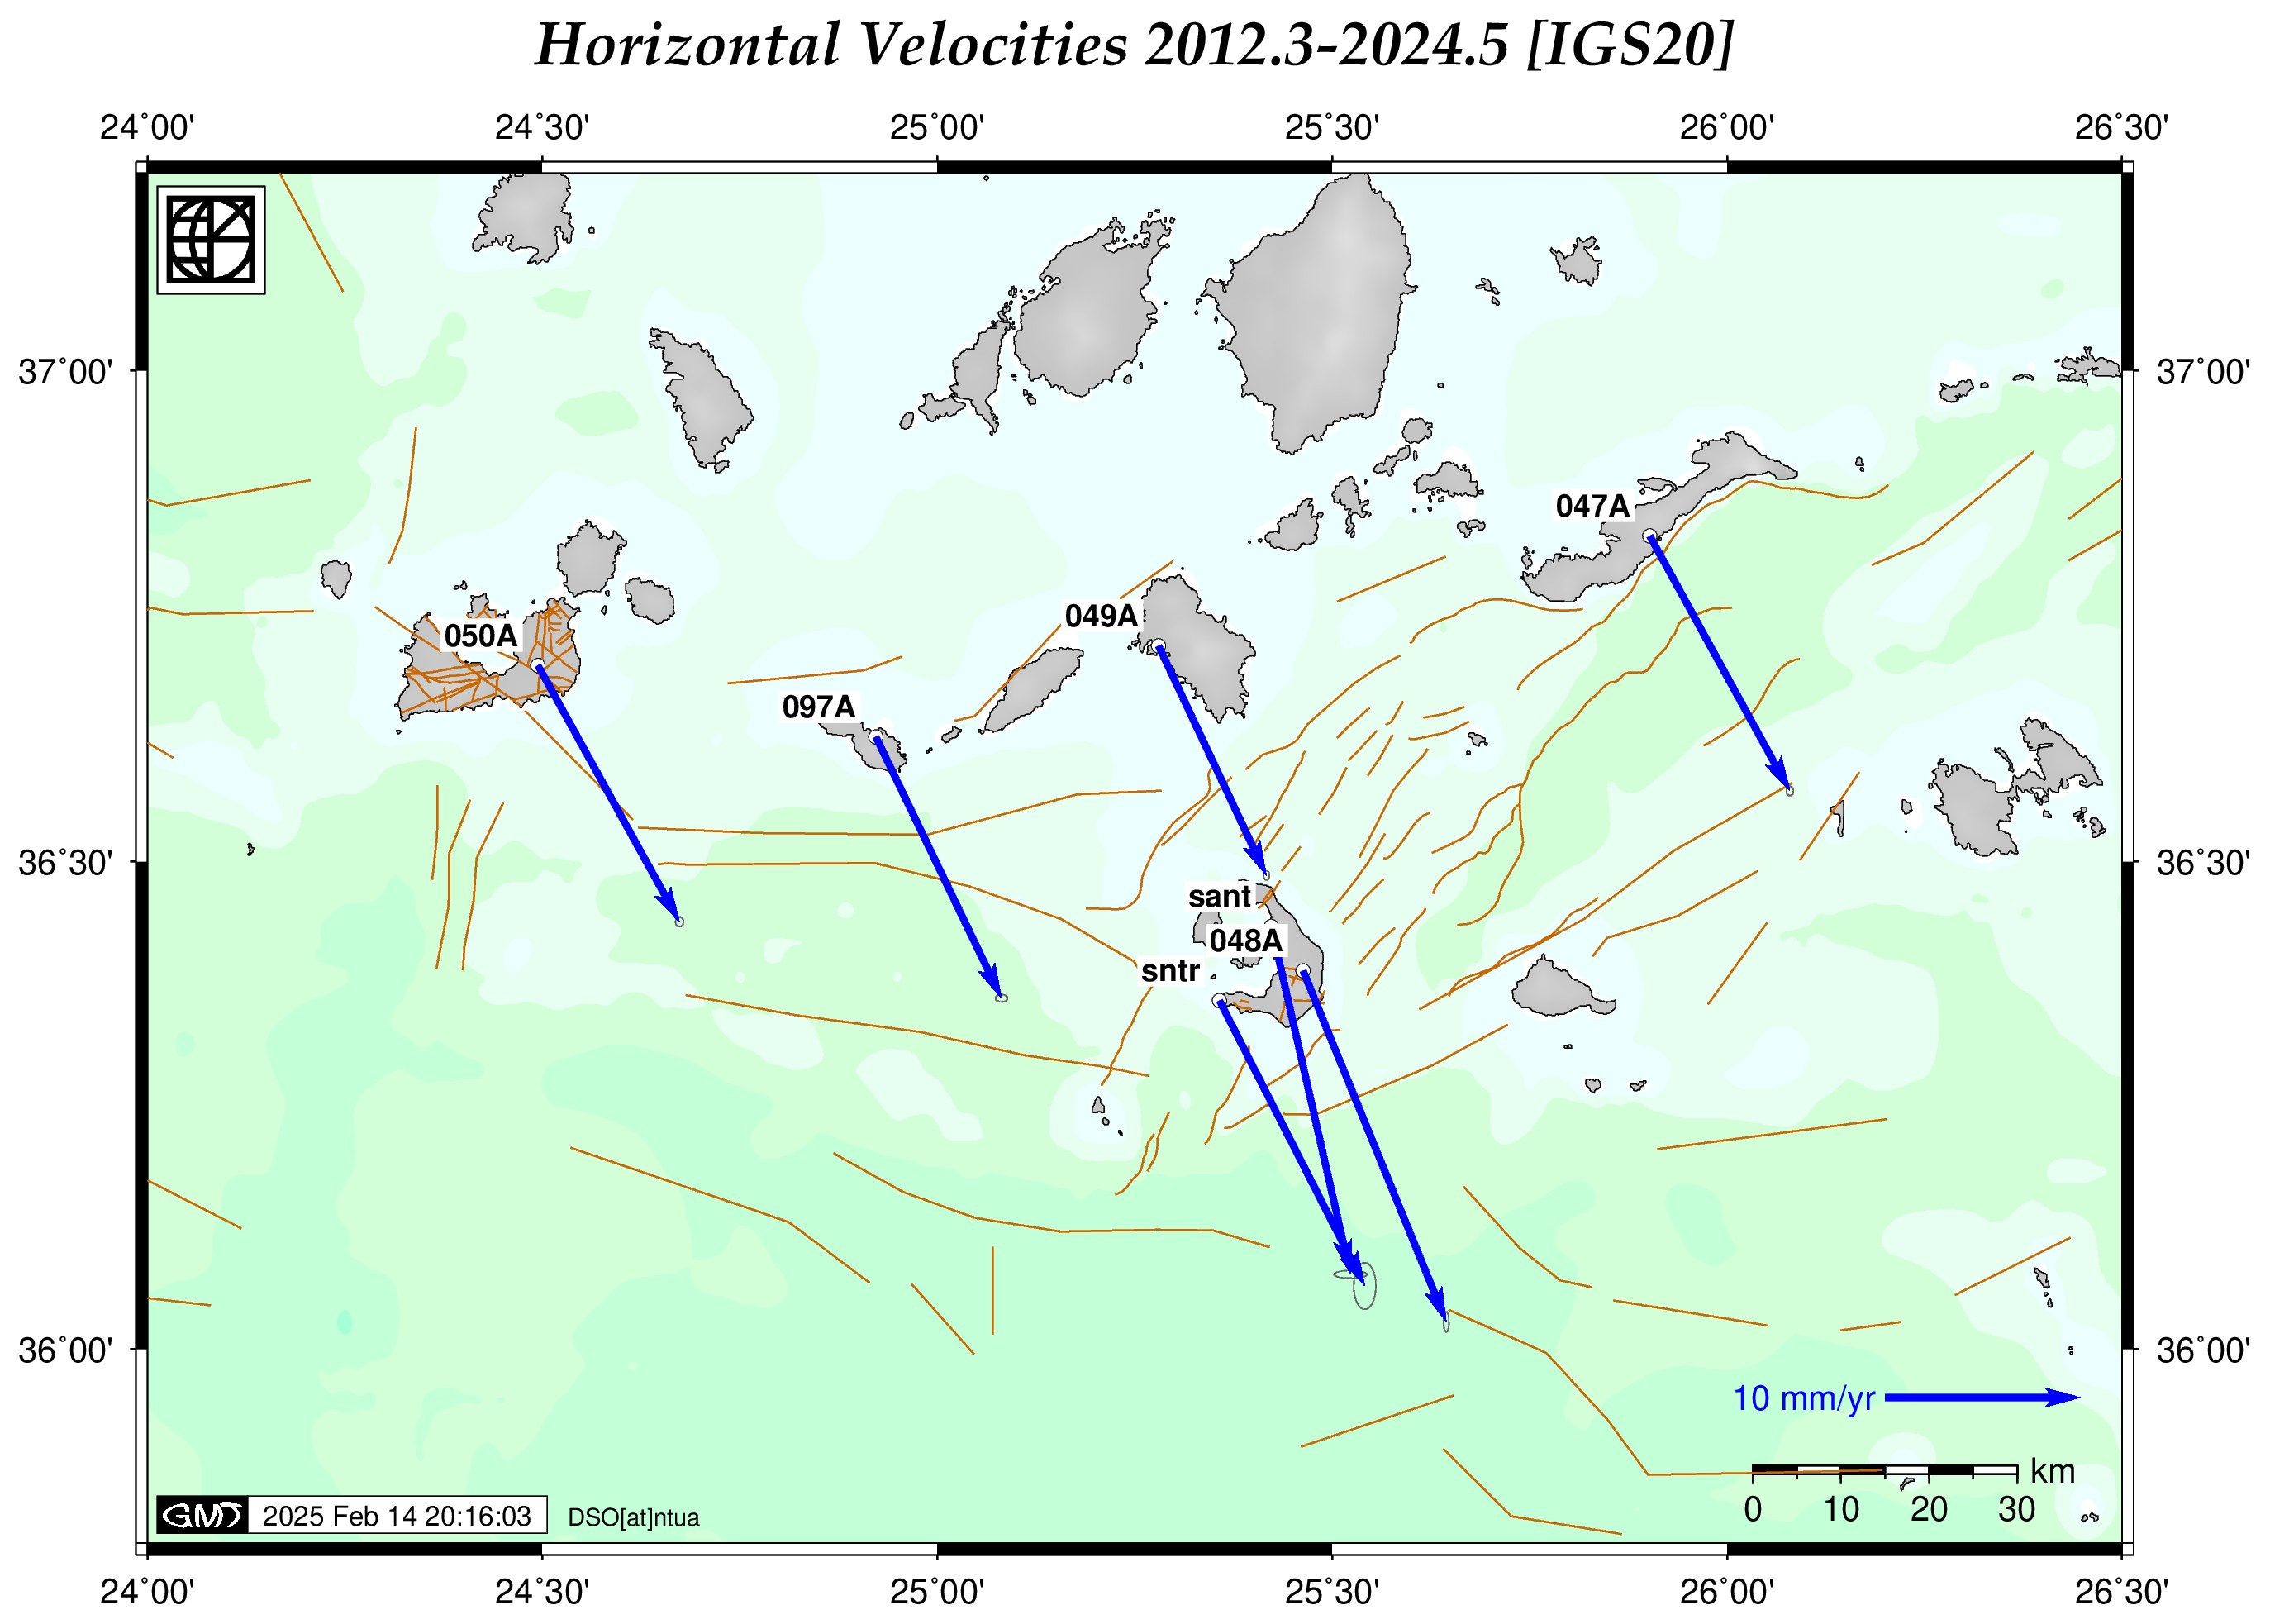
\includegraphics[width=.97\textwidth]{sant_1224_vhor.jpg}
      \end{center}  
    \end{column}
    \begin{column}{.5\textwidth}
      \begin{center}
        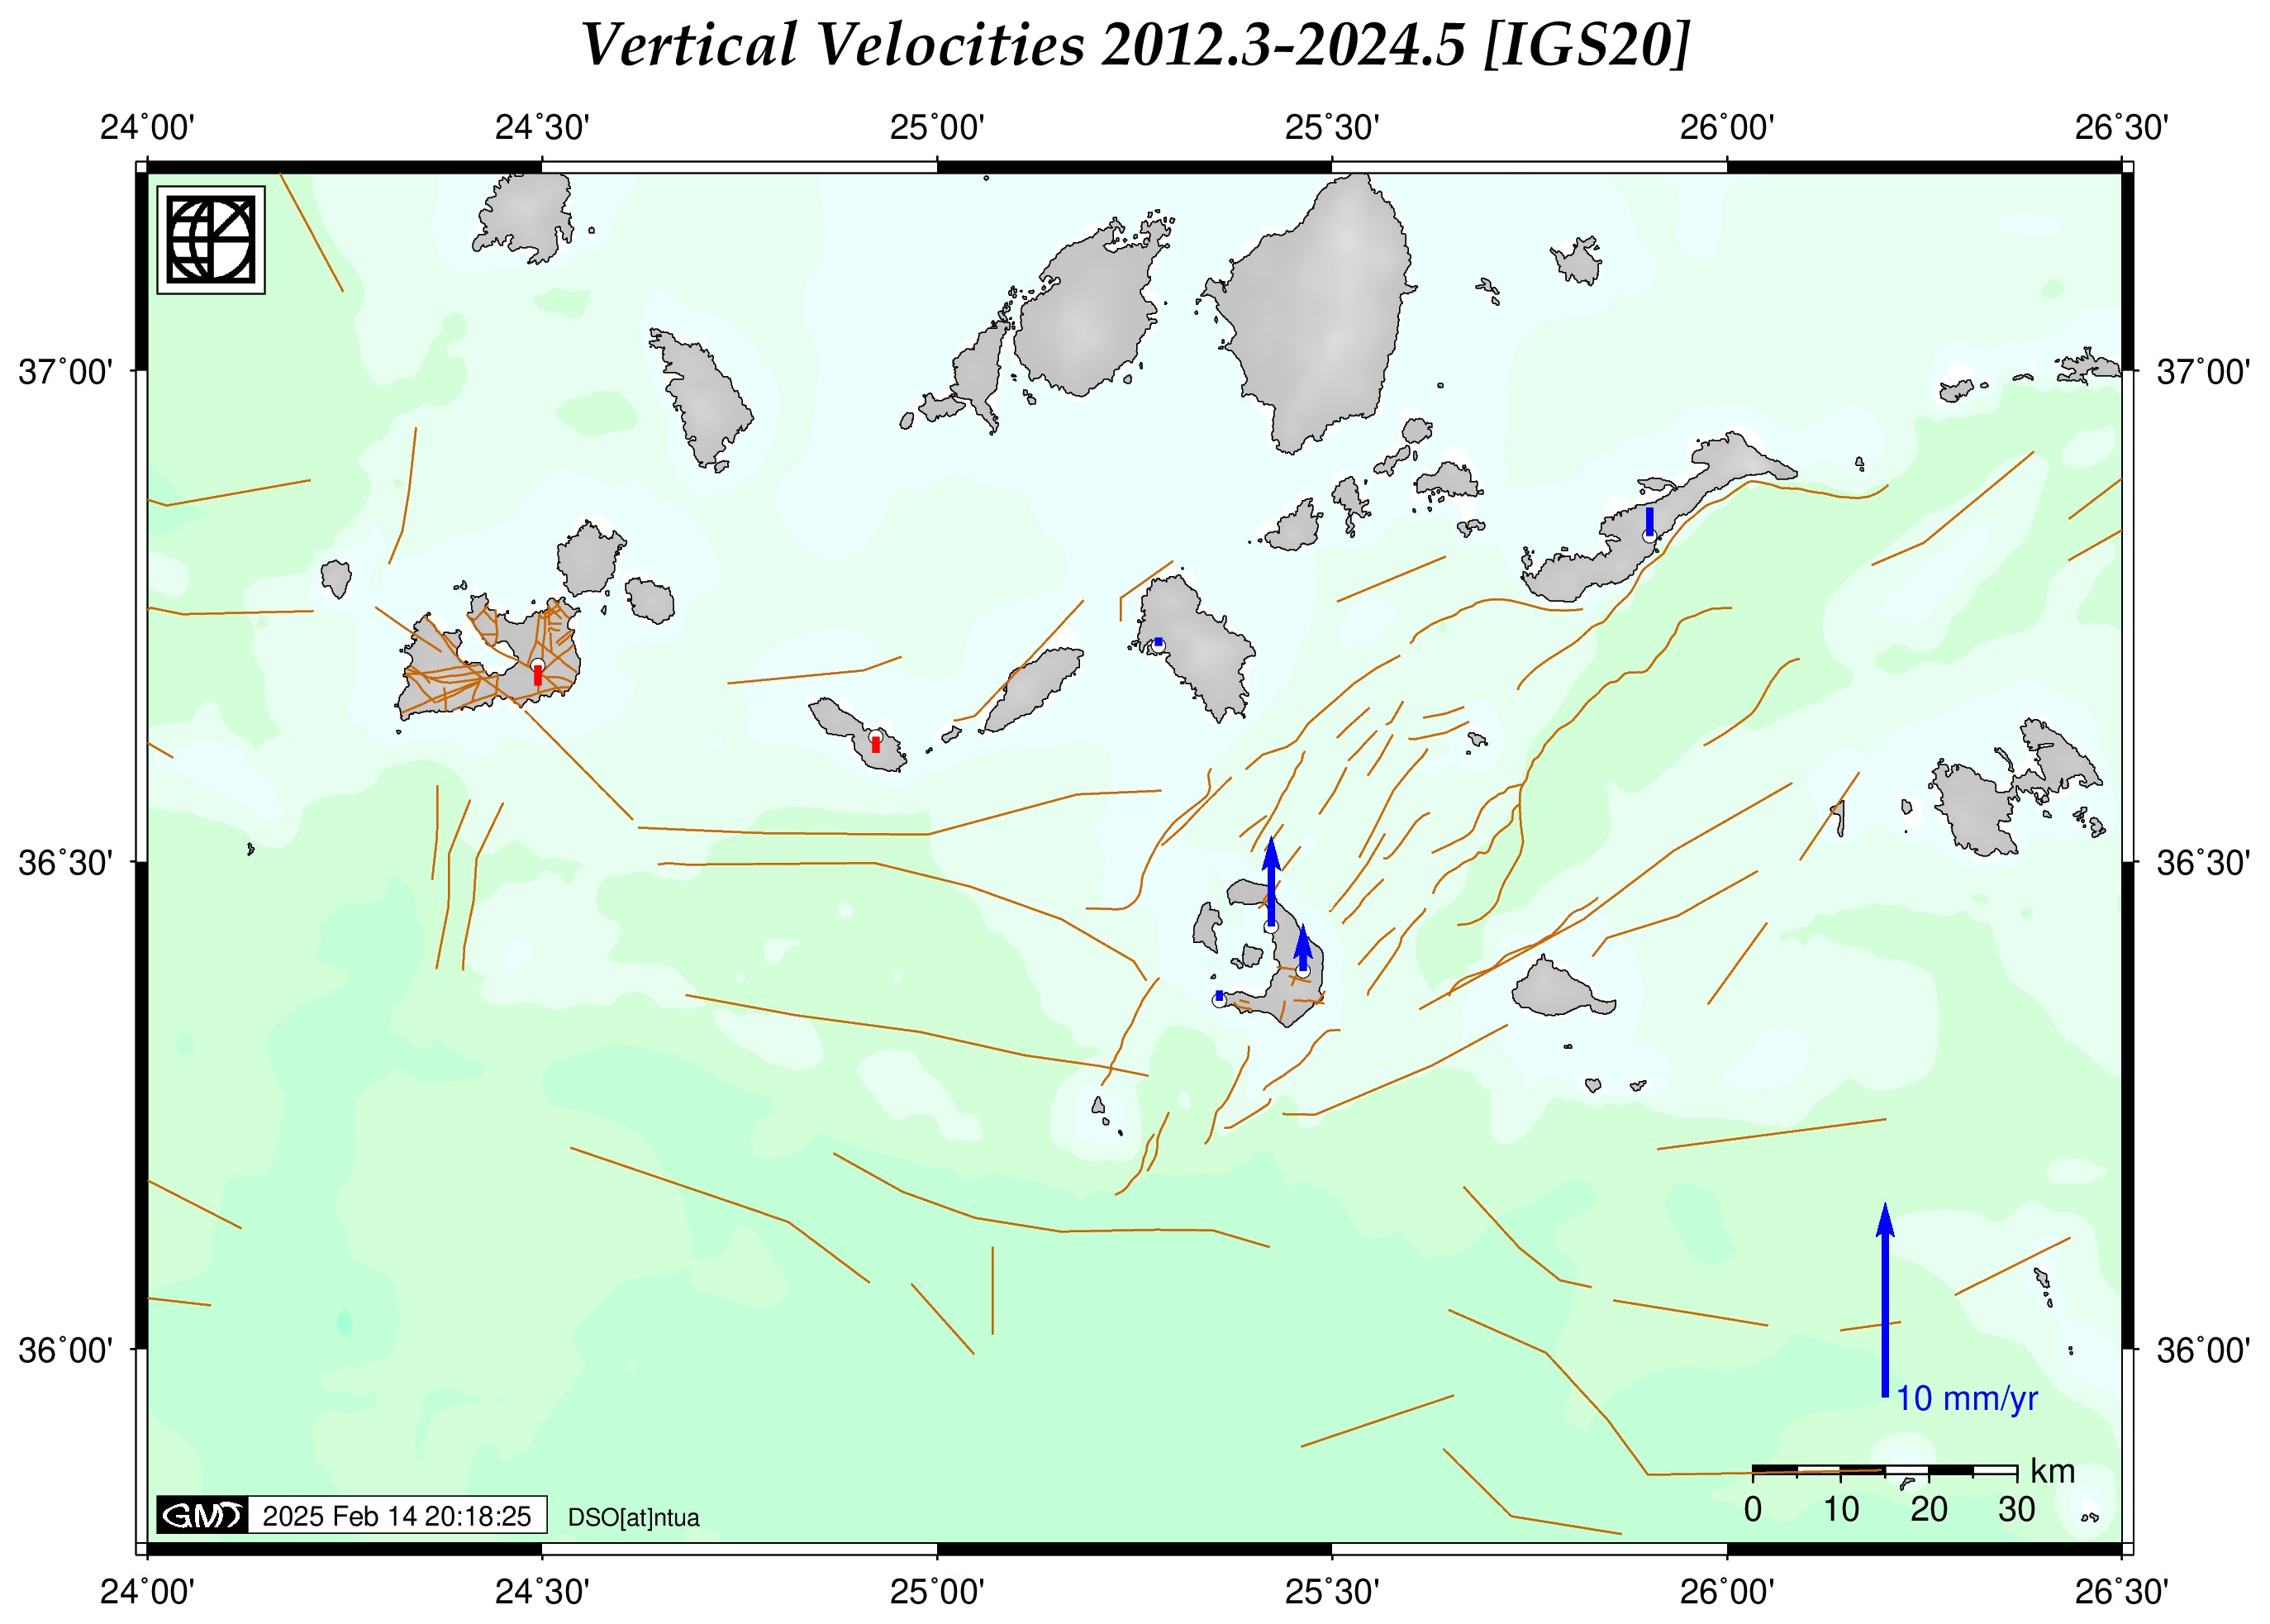
\includegraphics[width=.97\textwidth]{sant_1224_vver.jpg}
      \end{center}       
    \end{column}
  \end{columns}
~\\[1em]   
  \begin{tiny}
  \begin{itemize}\setlength\itemsep{.1em}
    \item[*] Mapping production: Generic Mapping Tools \citep{gmt}
    \item[*] Background: ETOPO1 \citep{etopo1}
    \item[*] Faults database: NOAfaults v6.0 \citep{noafaults}
  \end{itemize}
  \end{tiny}  
 
\end{frame}
\note{}

 % ------------------------------------------------------------------------------
\begin{frame}
  \frametitle{Station displacements 2024.6 - 2025.1 }
  \framesubtitle{}
  \label{}
  \vskip-.5cm
  \begin{columns}[T]
    \begin{column}{.5\textwidth}
      \begin{center}
        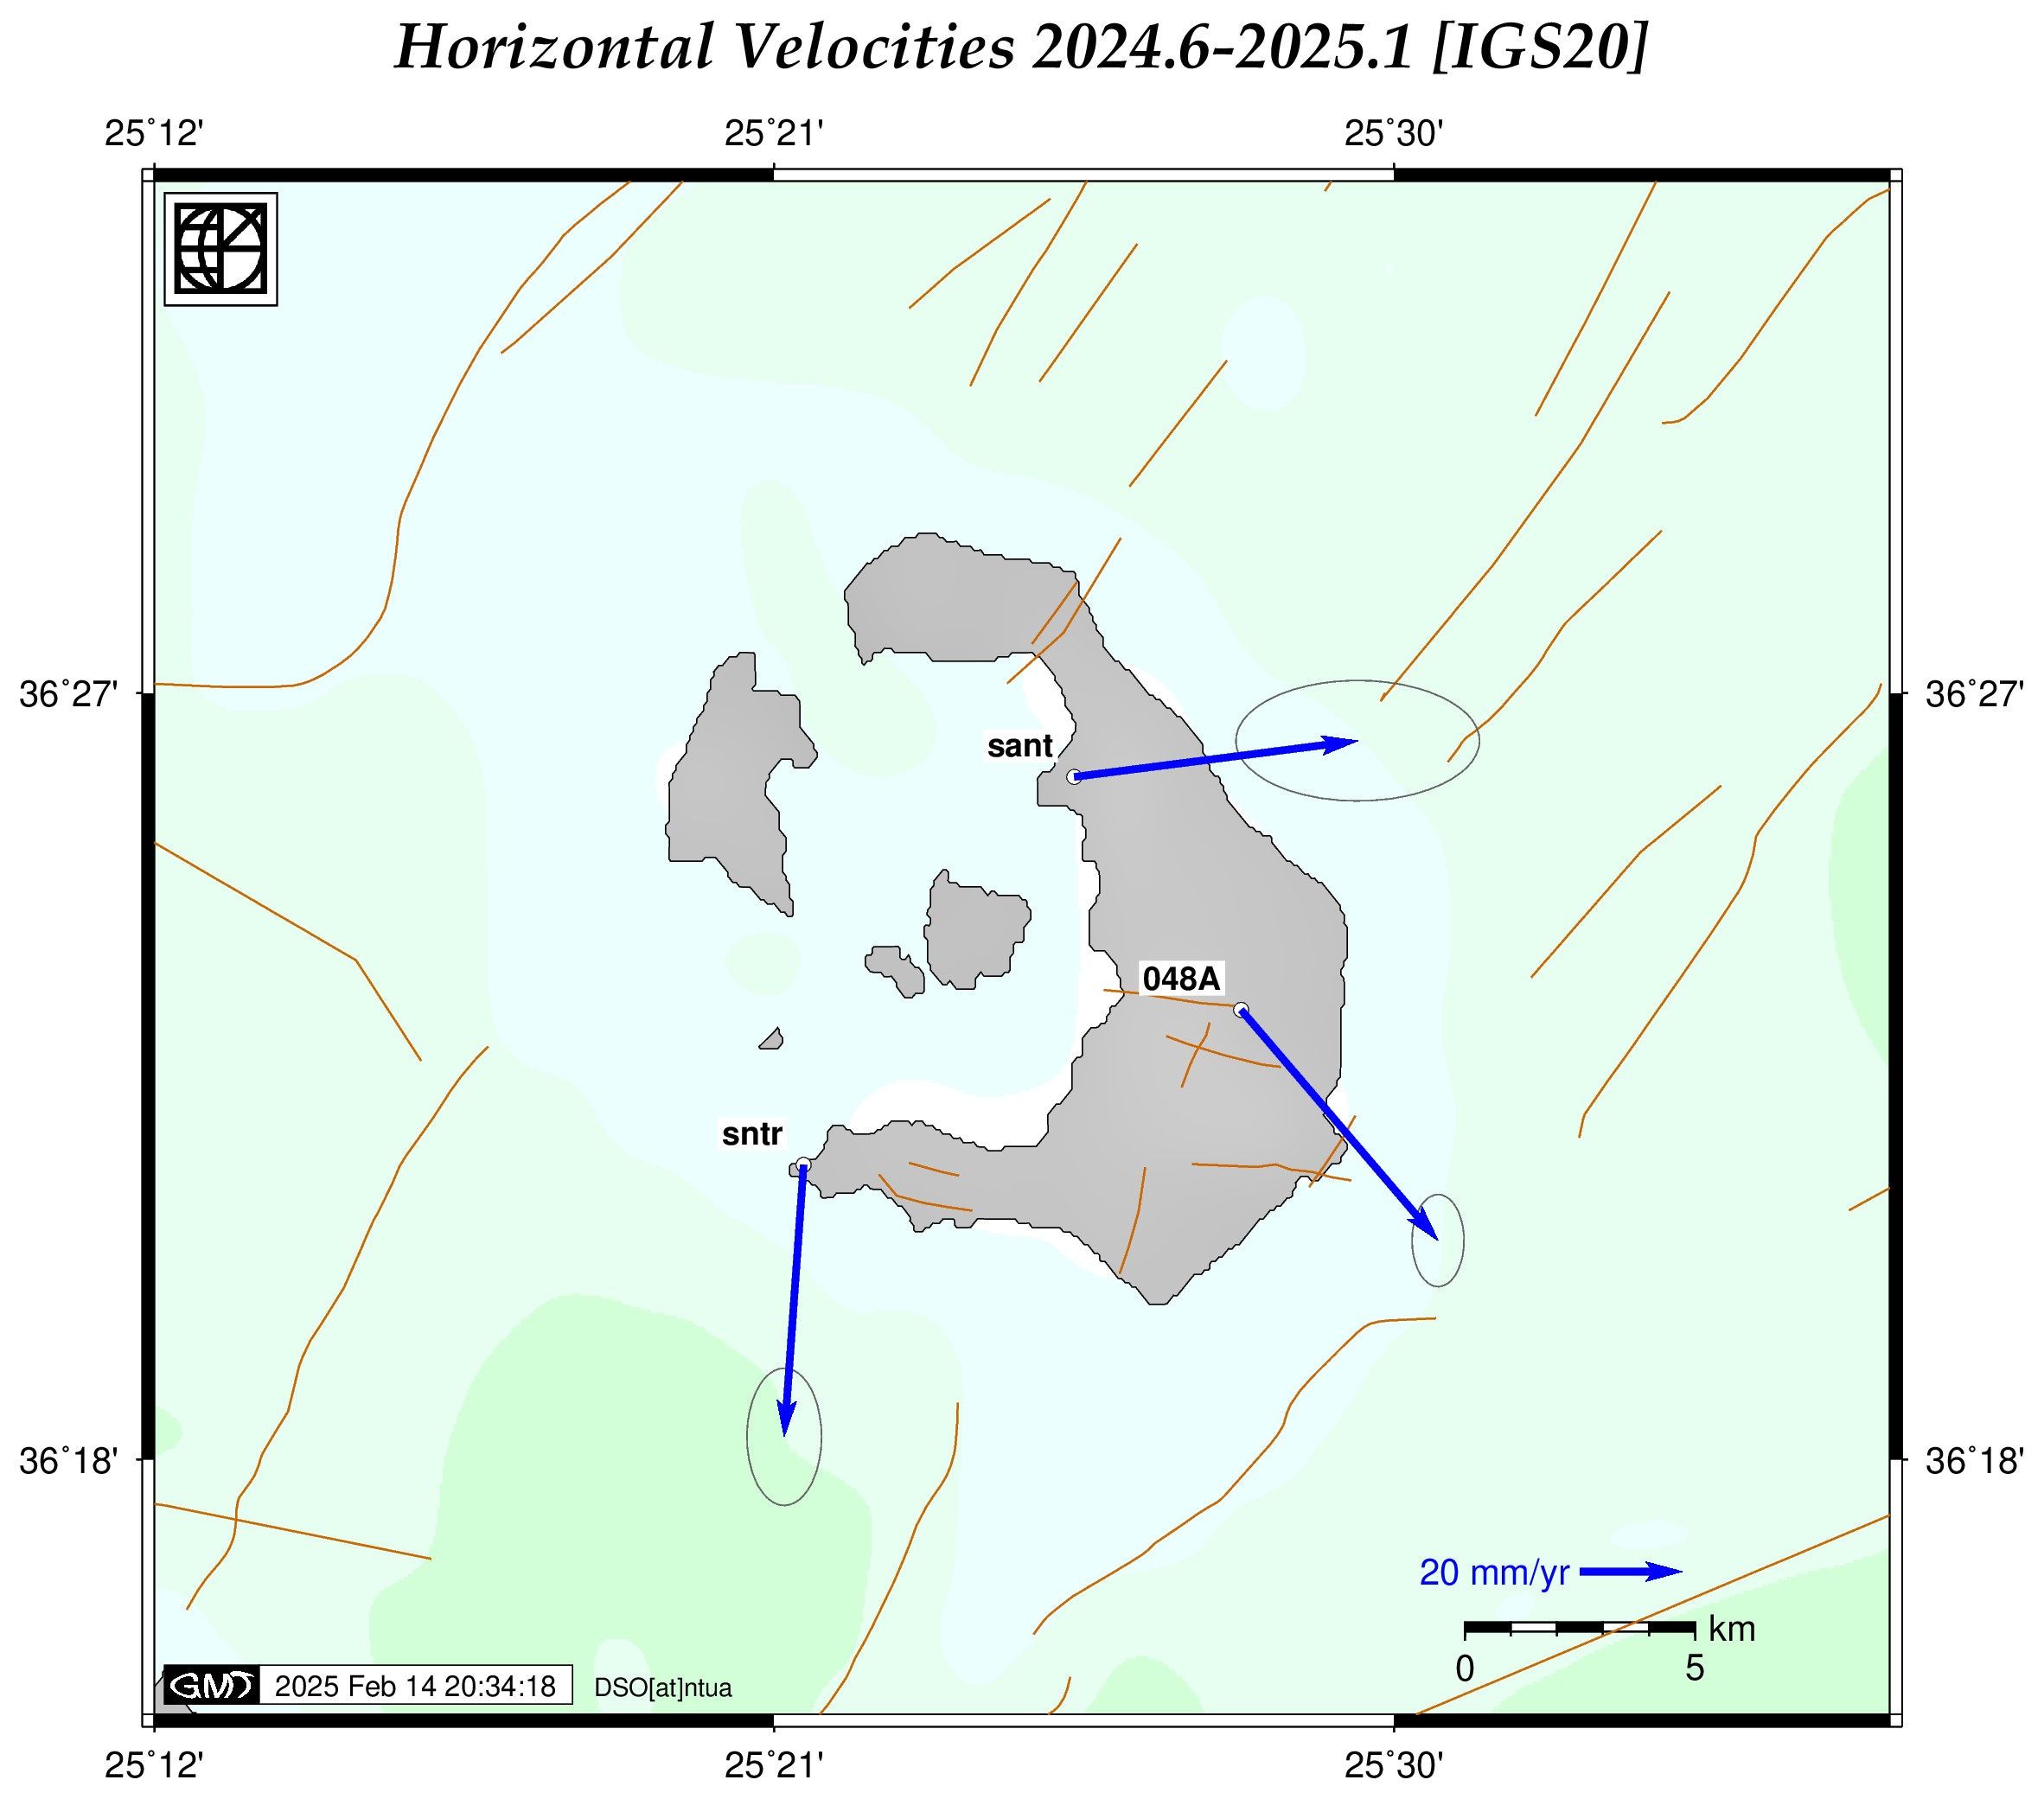
\includegraphics[width=.97\textwidth]{sant_2425_vhor.jpg}
      \end{center}  
    \end{column}
    \begin{column}{.5\textwidth}
      \begin{center}
        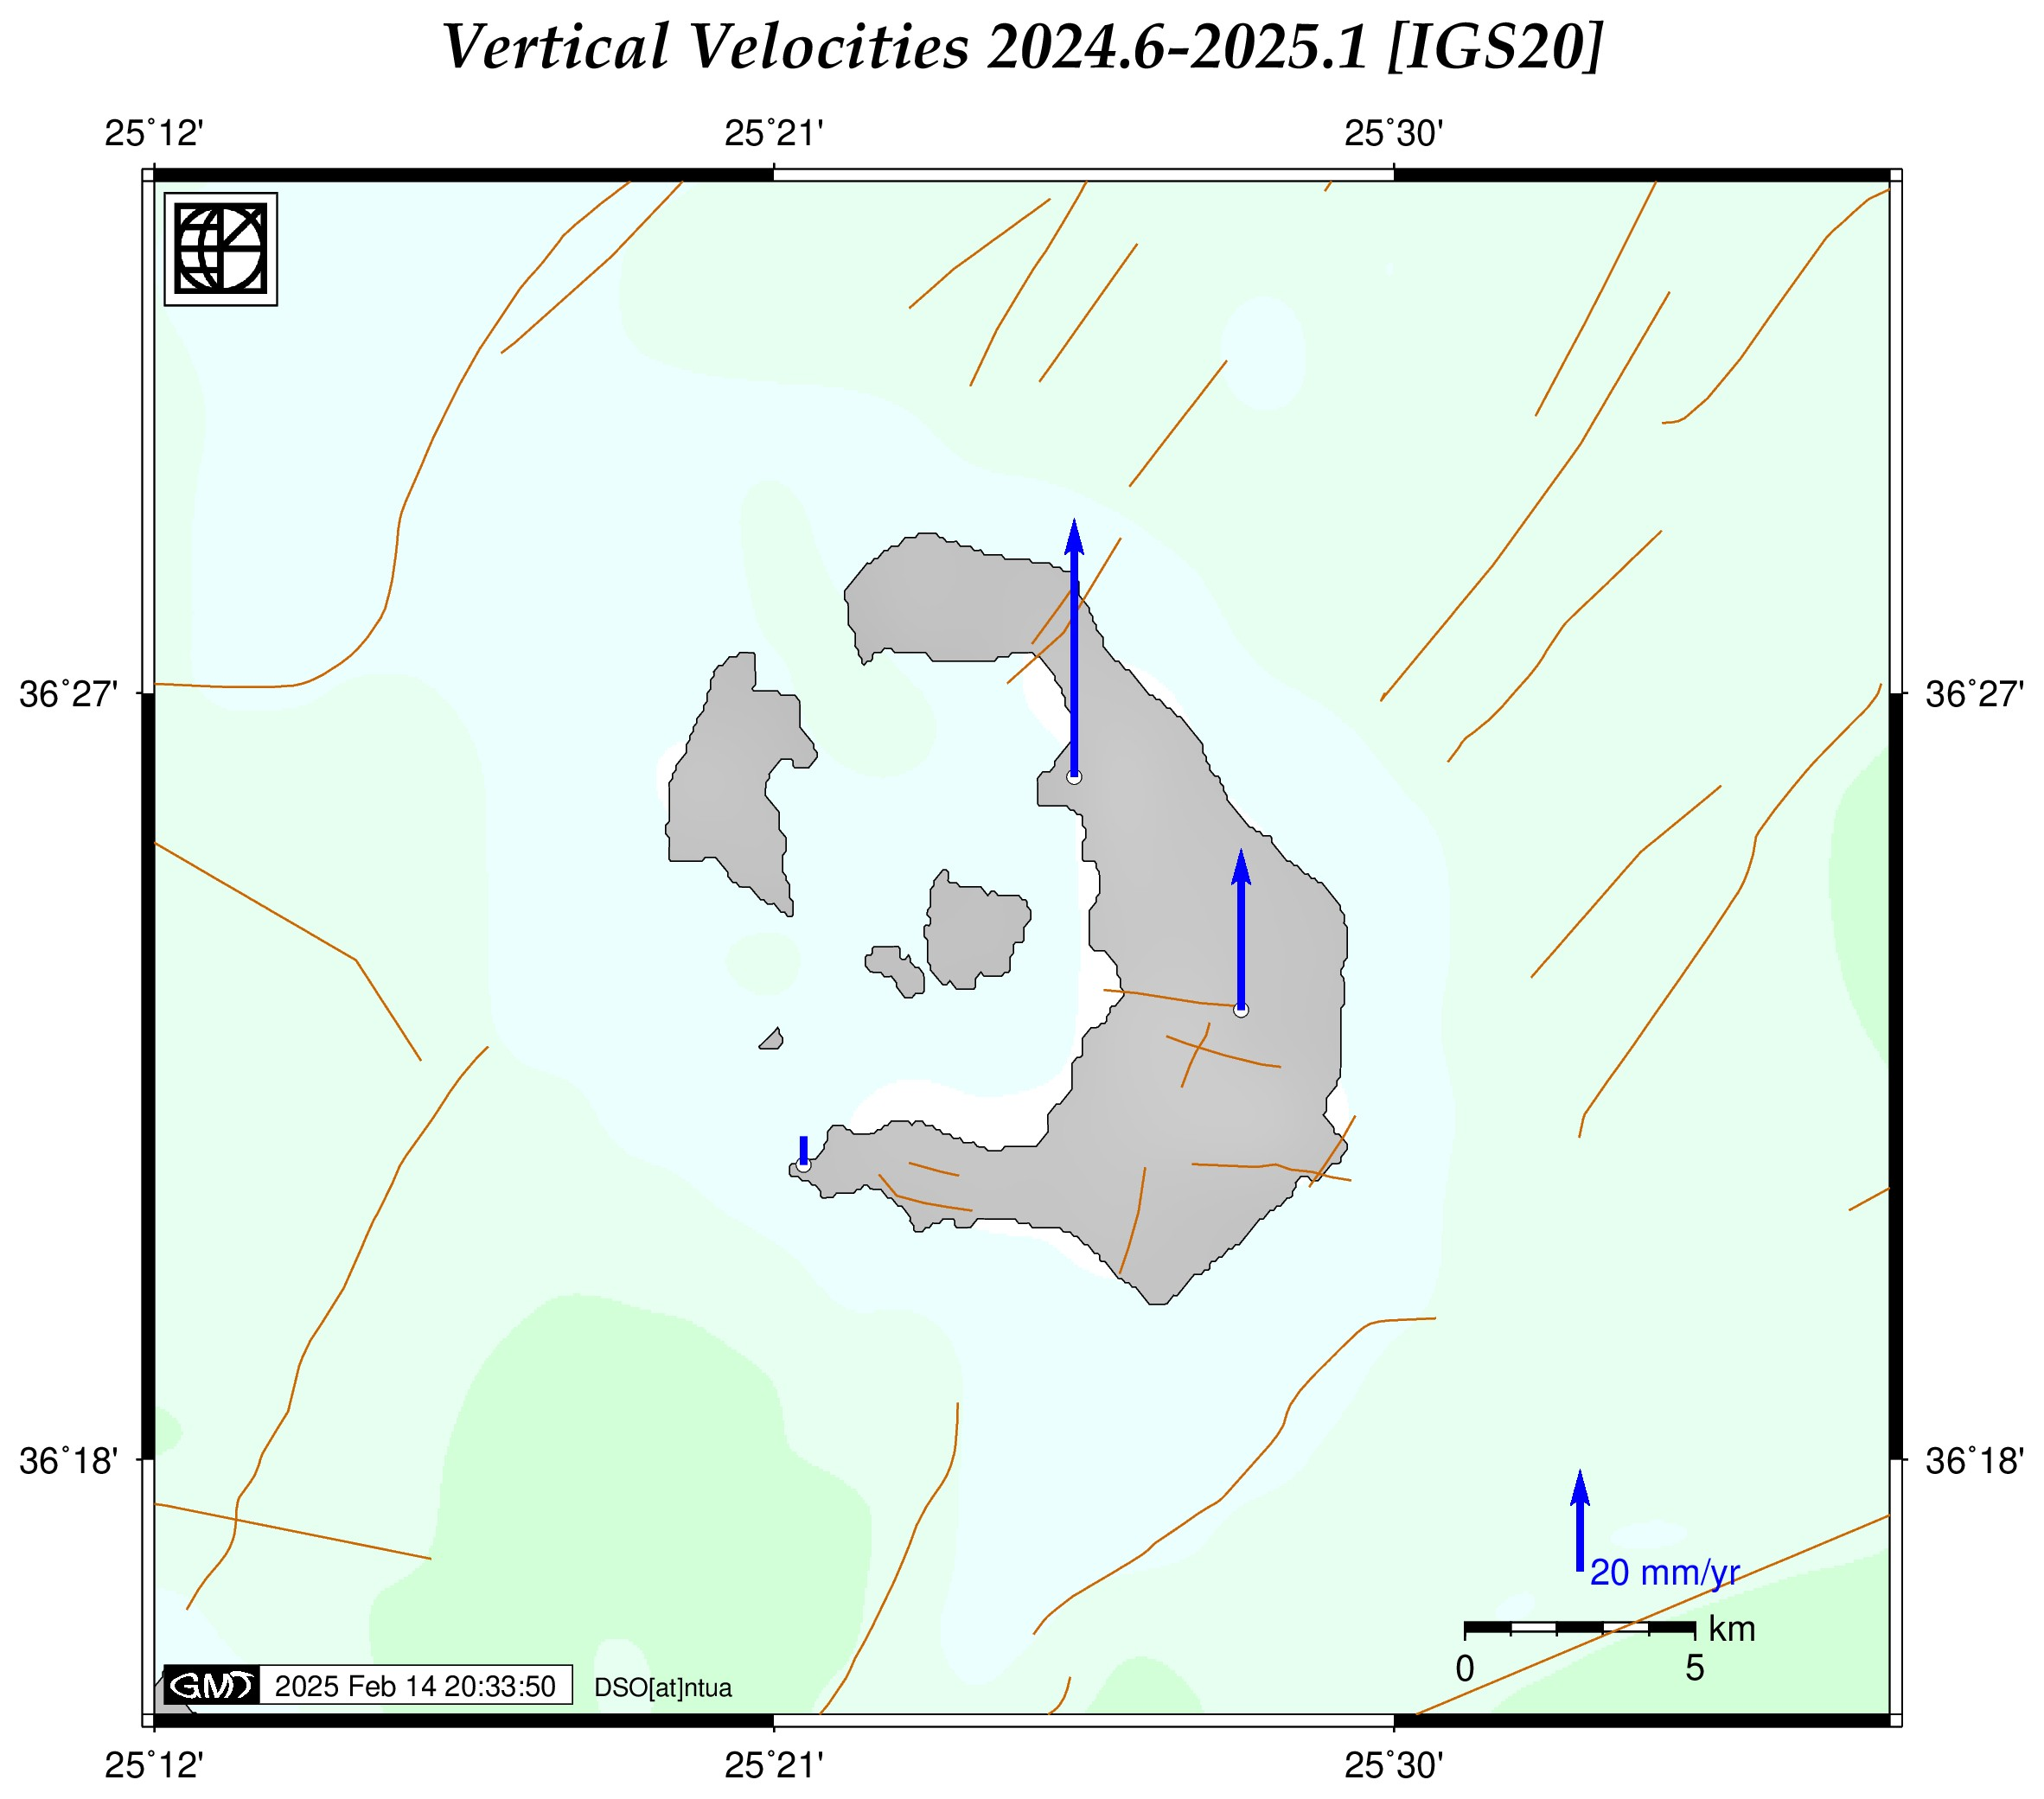
\includegraphics[width=.97\textwidth]{sant_2425_vver.jpg}
      \end{center}       
    \end{column}
  \end{columns}  

\end{frame}
\note{}

 % ------------------------------------------------------------------------------
\begin{frame}
  \frametitle{Time series analysis}
  \framesubtitle{}
  \label{}
  \begin{center}
  \vskip-.5cm
    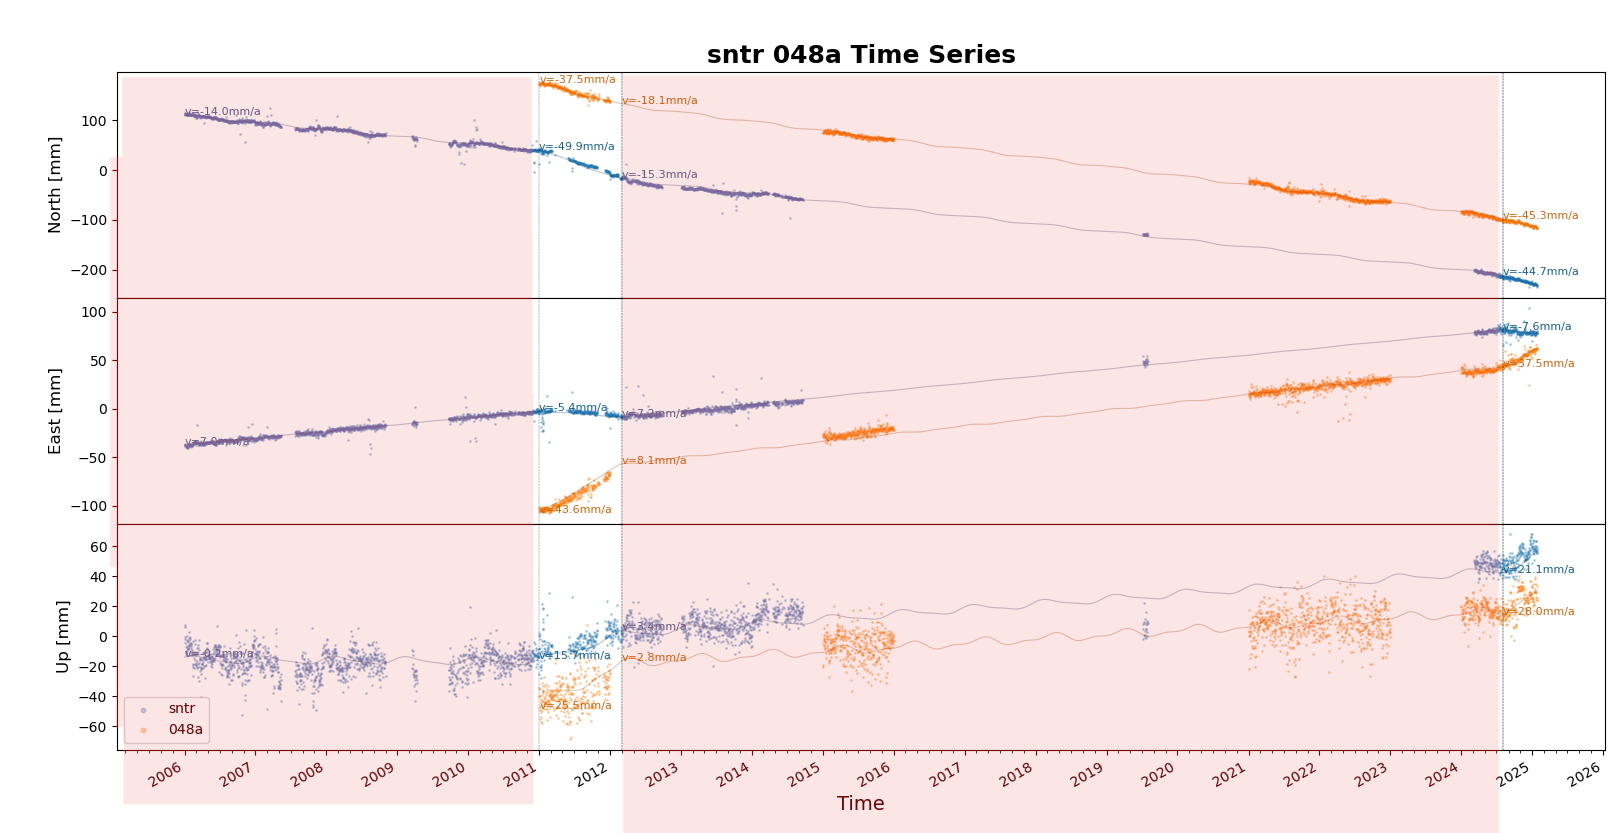
\includegraphics[width=.97\textwidth]{ts_sntr_048a.png}
  \end{center}
\end{frame}
\note{}




 % ------------------------------------------------------------------------------
\begin{frame}
  \frametitle{Time series analysis}
  \framesubtitle{}
  \label{}
  \vskip-1cm
  \begin{columns}[T]
    \begin{column}{.5\textwidth}
      \begin{center}
      {\scriptsize SANT}
        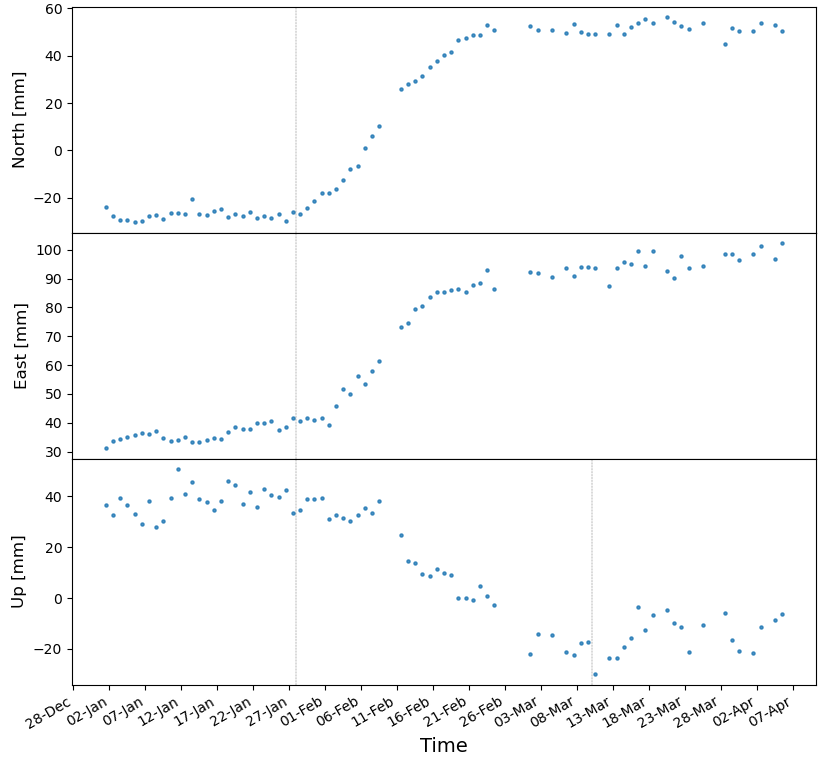
\includegraphics[width=.97\textwidth]{ts_snt2.png}
      \end{center}  
    \end{column}
    \begin{column}{.5\textwidth}
      \begin{center}
       {\scriptsize 048a}
        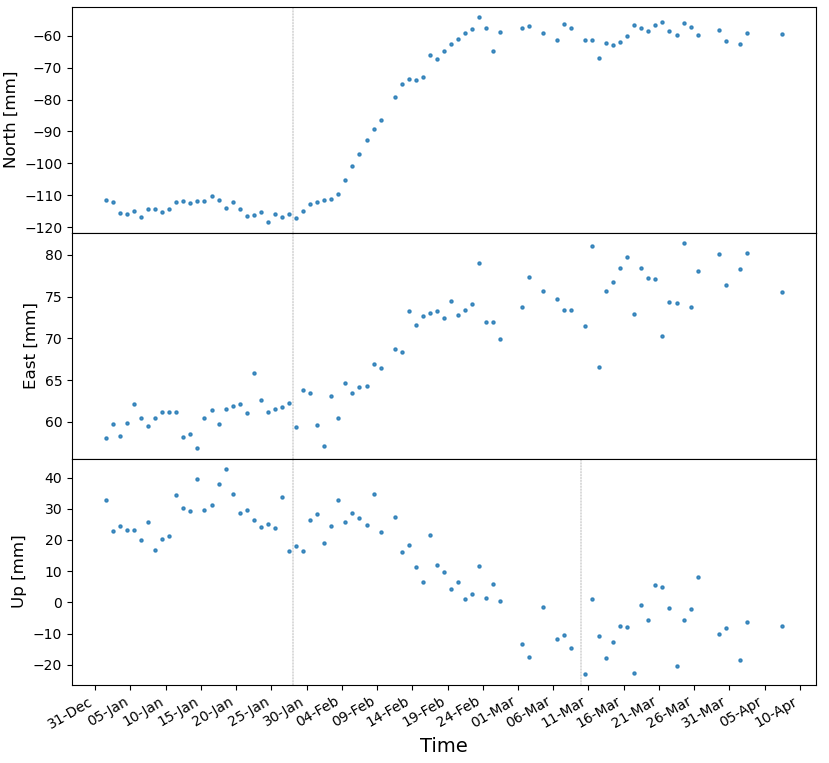
\includegraphics[width=.97\textwidth]{ts_048a.png}
      \end{center}       
    \end{column}
%  \begin{column}{.33\textwidth}
%      \begin{center}
%       {\scriptsize SNTR}
%        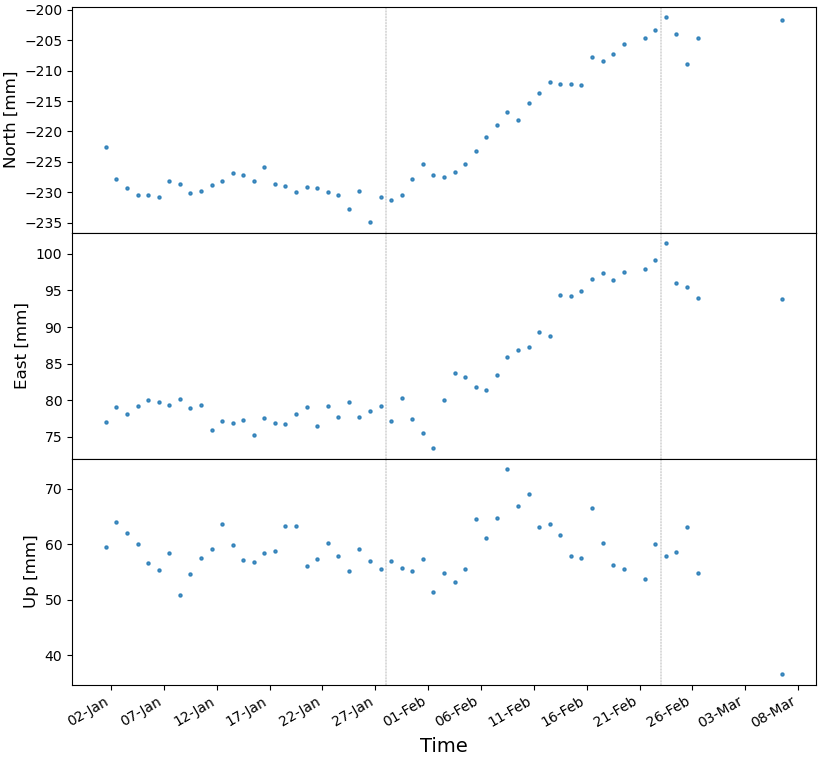
\includegraphics[width=.97\textwidth]{ts_sntr.png}
%      \end{center}  
%    \end{column}
  \end{columns}  
  
\end{frame}
\note{}

 % ------------------------------------------------------------------------------
\begin{frame}
  \frametitle{Time series analysis}
  \framesubtitle{}
  \label{}
  \vskip-1cm
  \begin{columns}[T]
    \begin{column}{.5\textwidth}
      \begin{center}
      {\scriptsize SANT}
        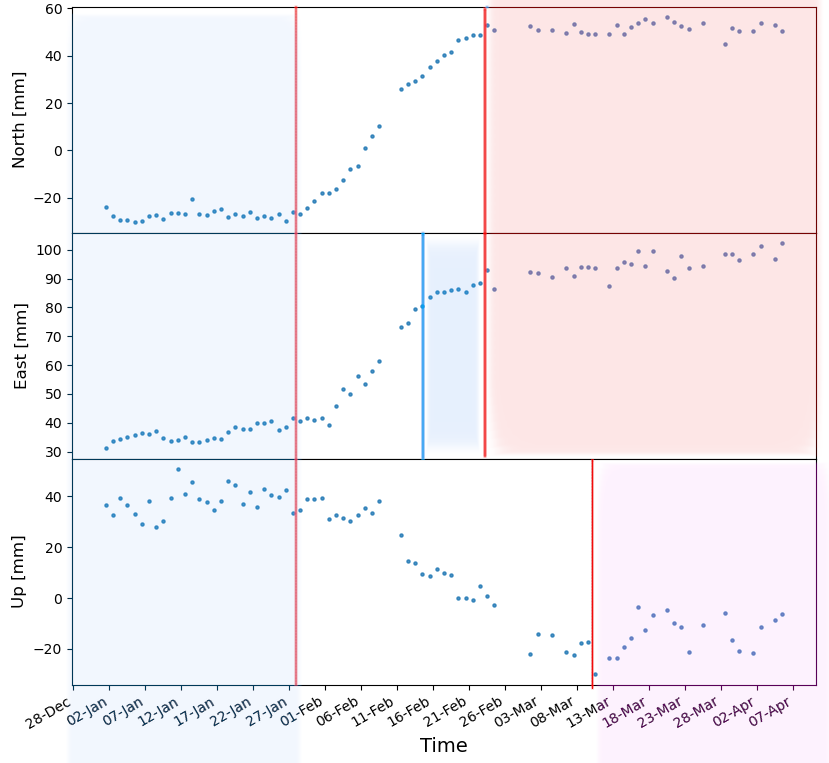
\includegraphics[width=.97\textwidth]{ts_snt2_mod.png}
      \end{center}  
    \end{column}
    \begin{column}{.5\textwidth}
      \begin{center}
       {\scriptsize 048a}
        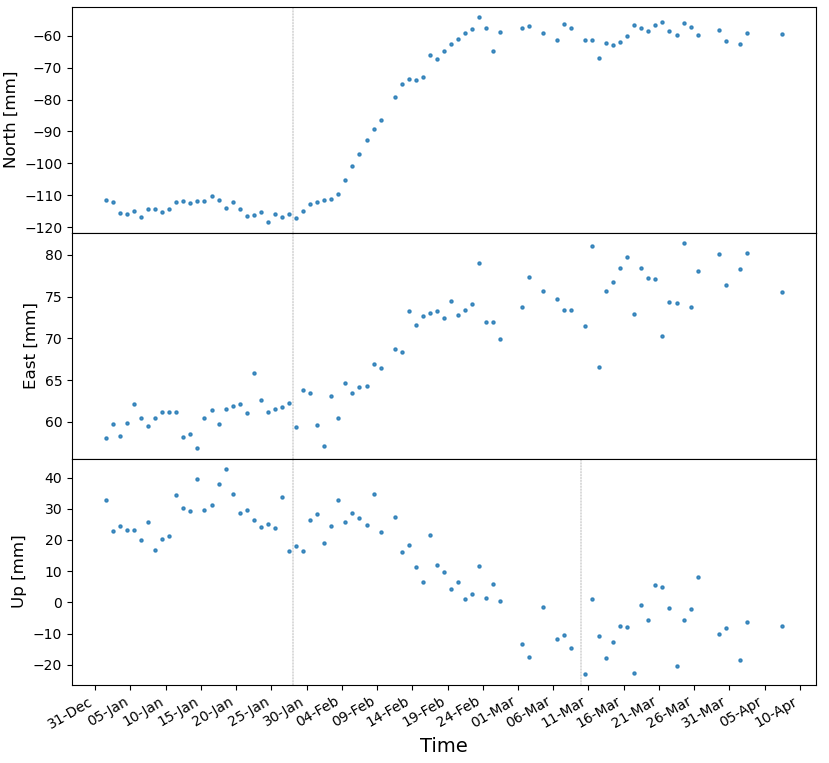
\includegraphics[width=.97\textwidth]{ts_048a.png}
      \end{center}       
    \end{column}
%  \begin{column}{.33\textwidth}
%      \begin{center}
%       {\scriptsize SNTR}
%        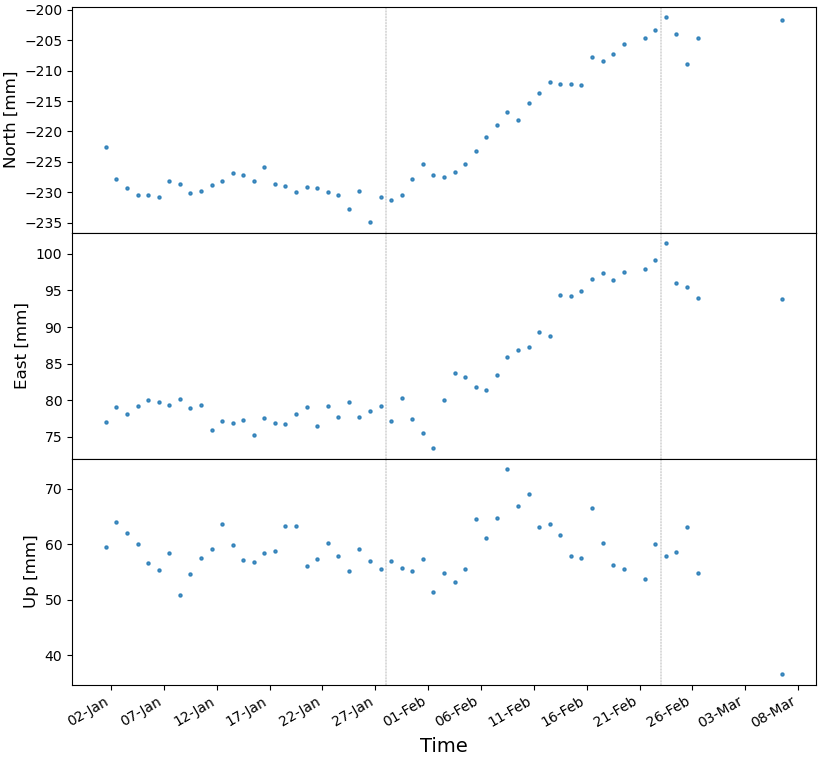
\includegraphics[width=.97\textwidth]{ts_sntr.png}
%      \end{center}  
%    \end{column}
  \end{columns}  
  
\end{frame}
\note{}

% ------------------------------------------------------------------------------
\begin{frame}
  \frametitle{Time series analysis}
  \framesubtitle{}
  \label{}
  \vskip-1cm
  \begin{columns}[T]
    \begin{column}{.5\textwidth}
      \begin{center}
      {\scriptsize 049a (Ίος)}
        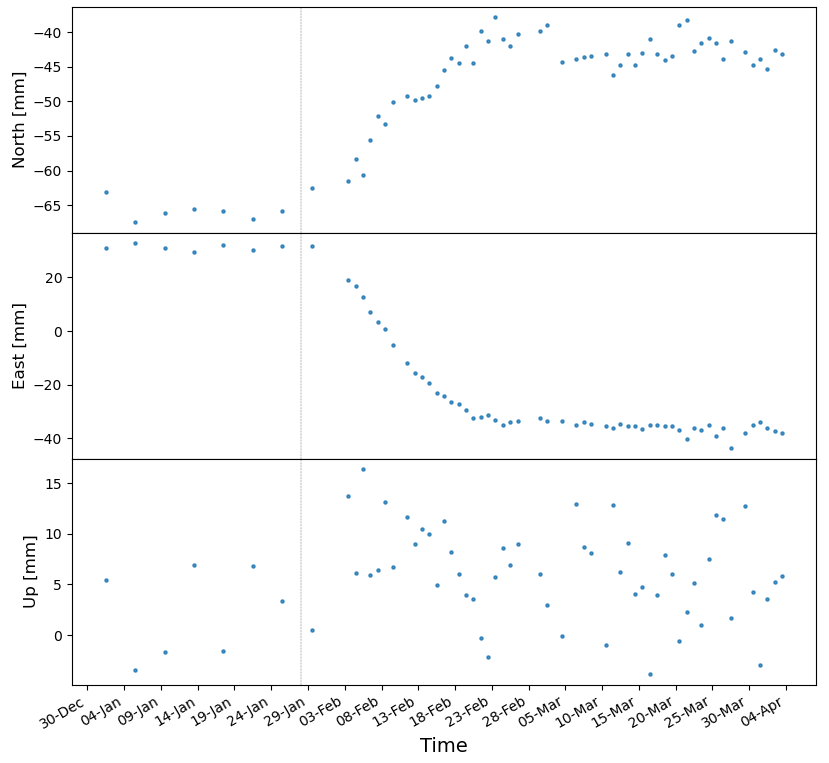
\includegraphics[width=.97\textwidth]{ts_049a.png}
      \end{center}  
    \end{column}
    \begin{column}{.5\textwidth}
      \begin{center}
       {\scriptsize ANYD}
        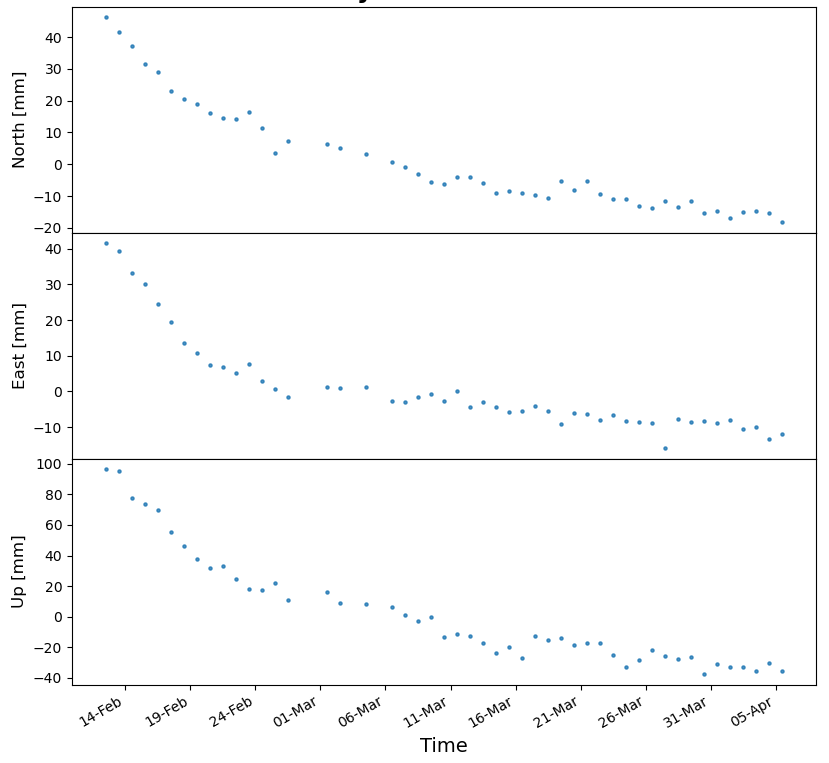
\includegraphics[width=.97\textwidth]{ts_anyd.png}
      \end{center}       
    \end{column}
%  \begin{column}{.33\textwidth}
%      \begin{center}
%       {\scriptsize SNTR}
%        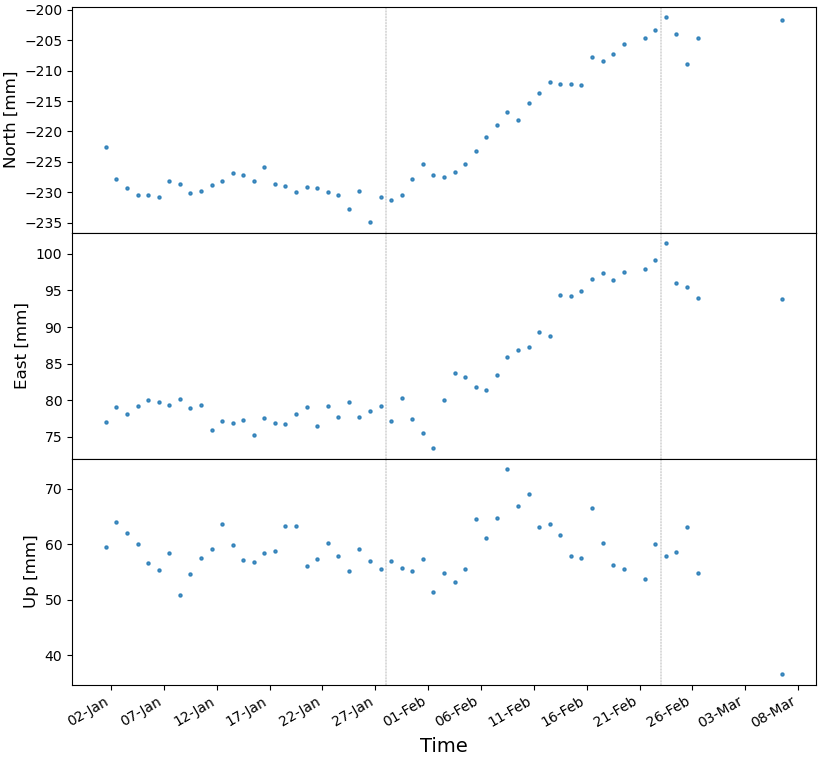
\includegraphics[width=.97\textwidth]{ts_sntr.png}
%      \end{center}  
%    \end{column}
  \end{columns}  
  
\end{frame}
\note{}

 % ------------------------------------------------------------------------------
\begin{frame}
  \frametitle{Station displacements 2025 28/1 - 16/2 }
  \framesubtitle{}
  \label{}
  \vskip-.5cm
  \begin{columns}[T]
    \begin{column}{.5\textwidth}
      \begin{center}
        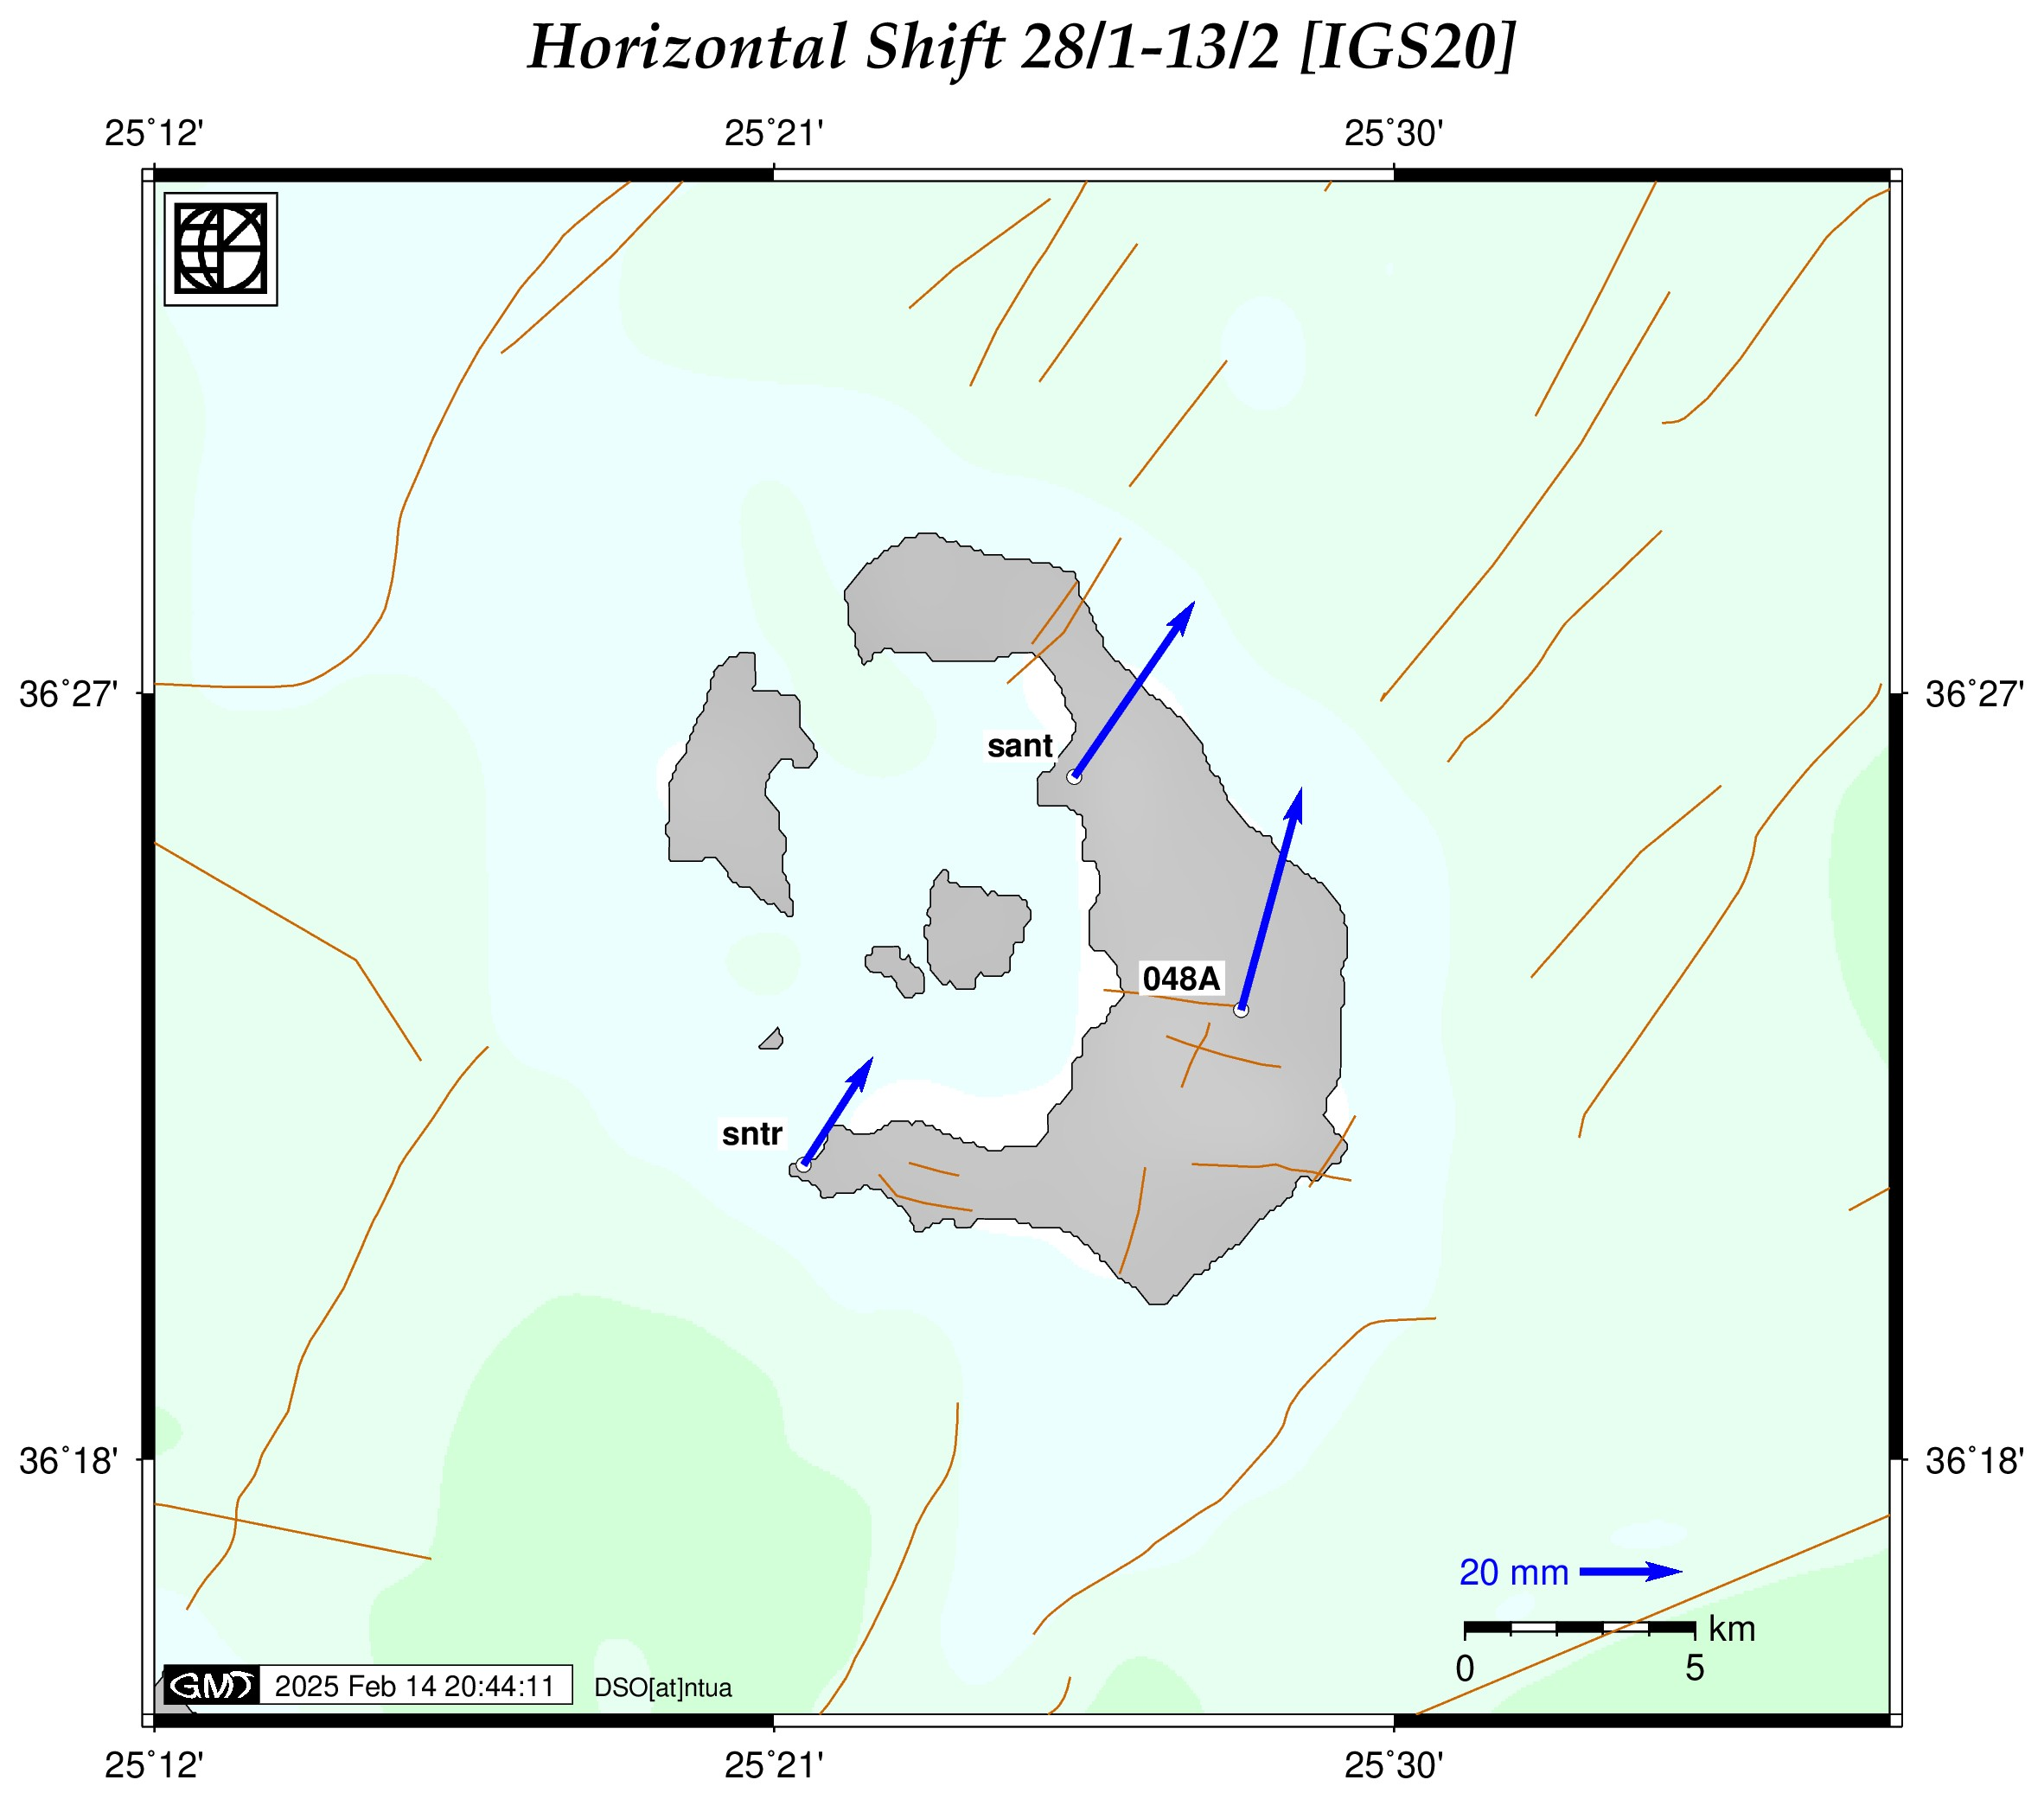
\includegraphics[width=.97\textwidth]{sant_2501_vhor.jpg}
      \end{center}  
    \end{column}
    \begin{column}{.5\textwidth}
      \begin{center}
        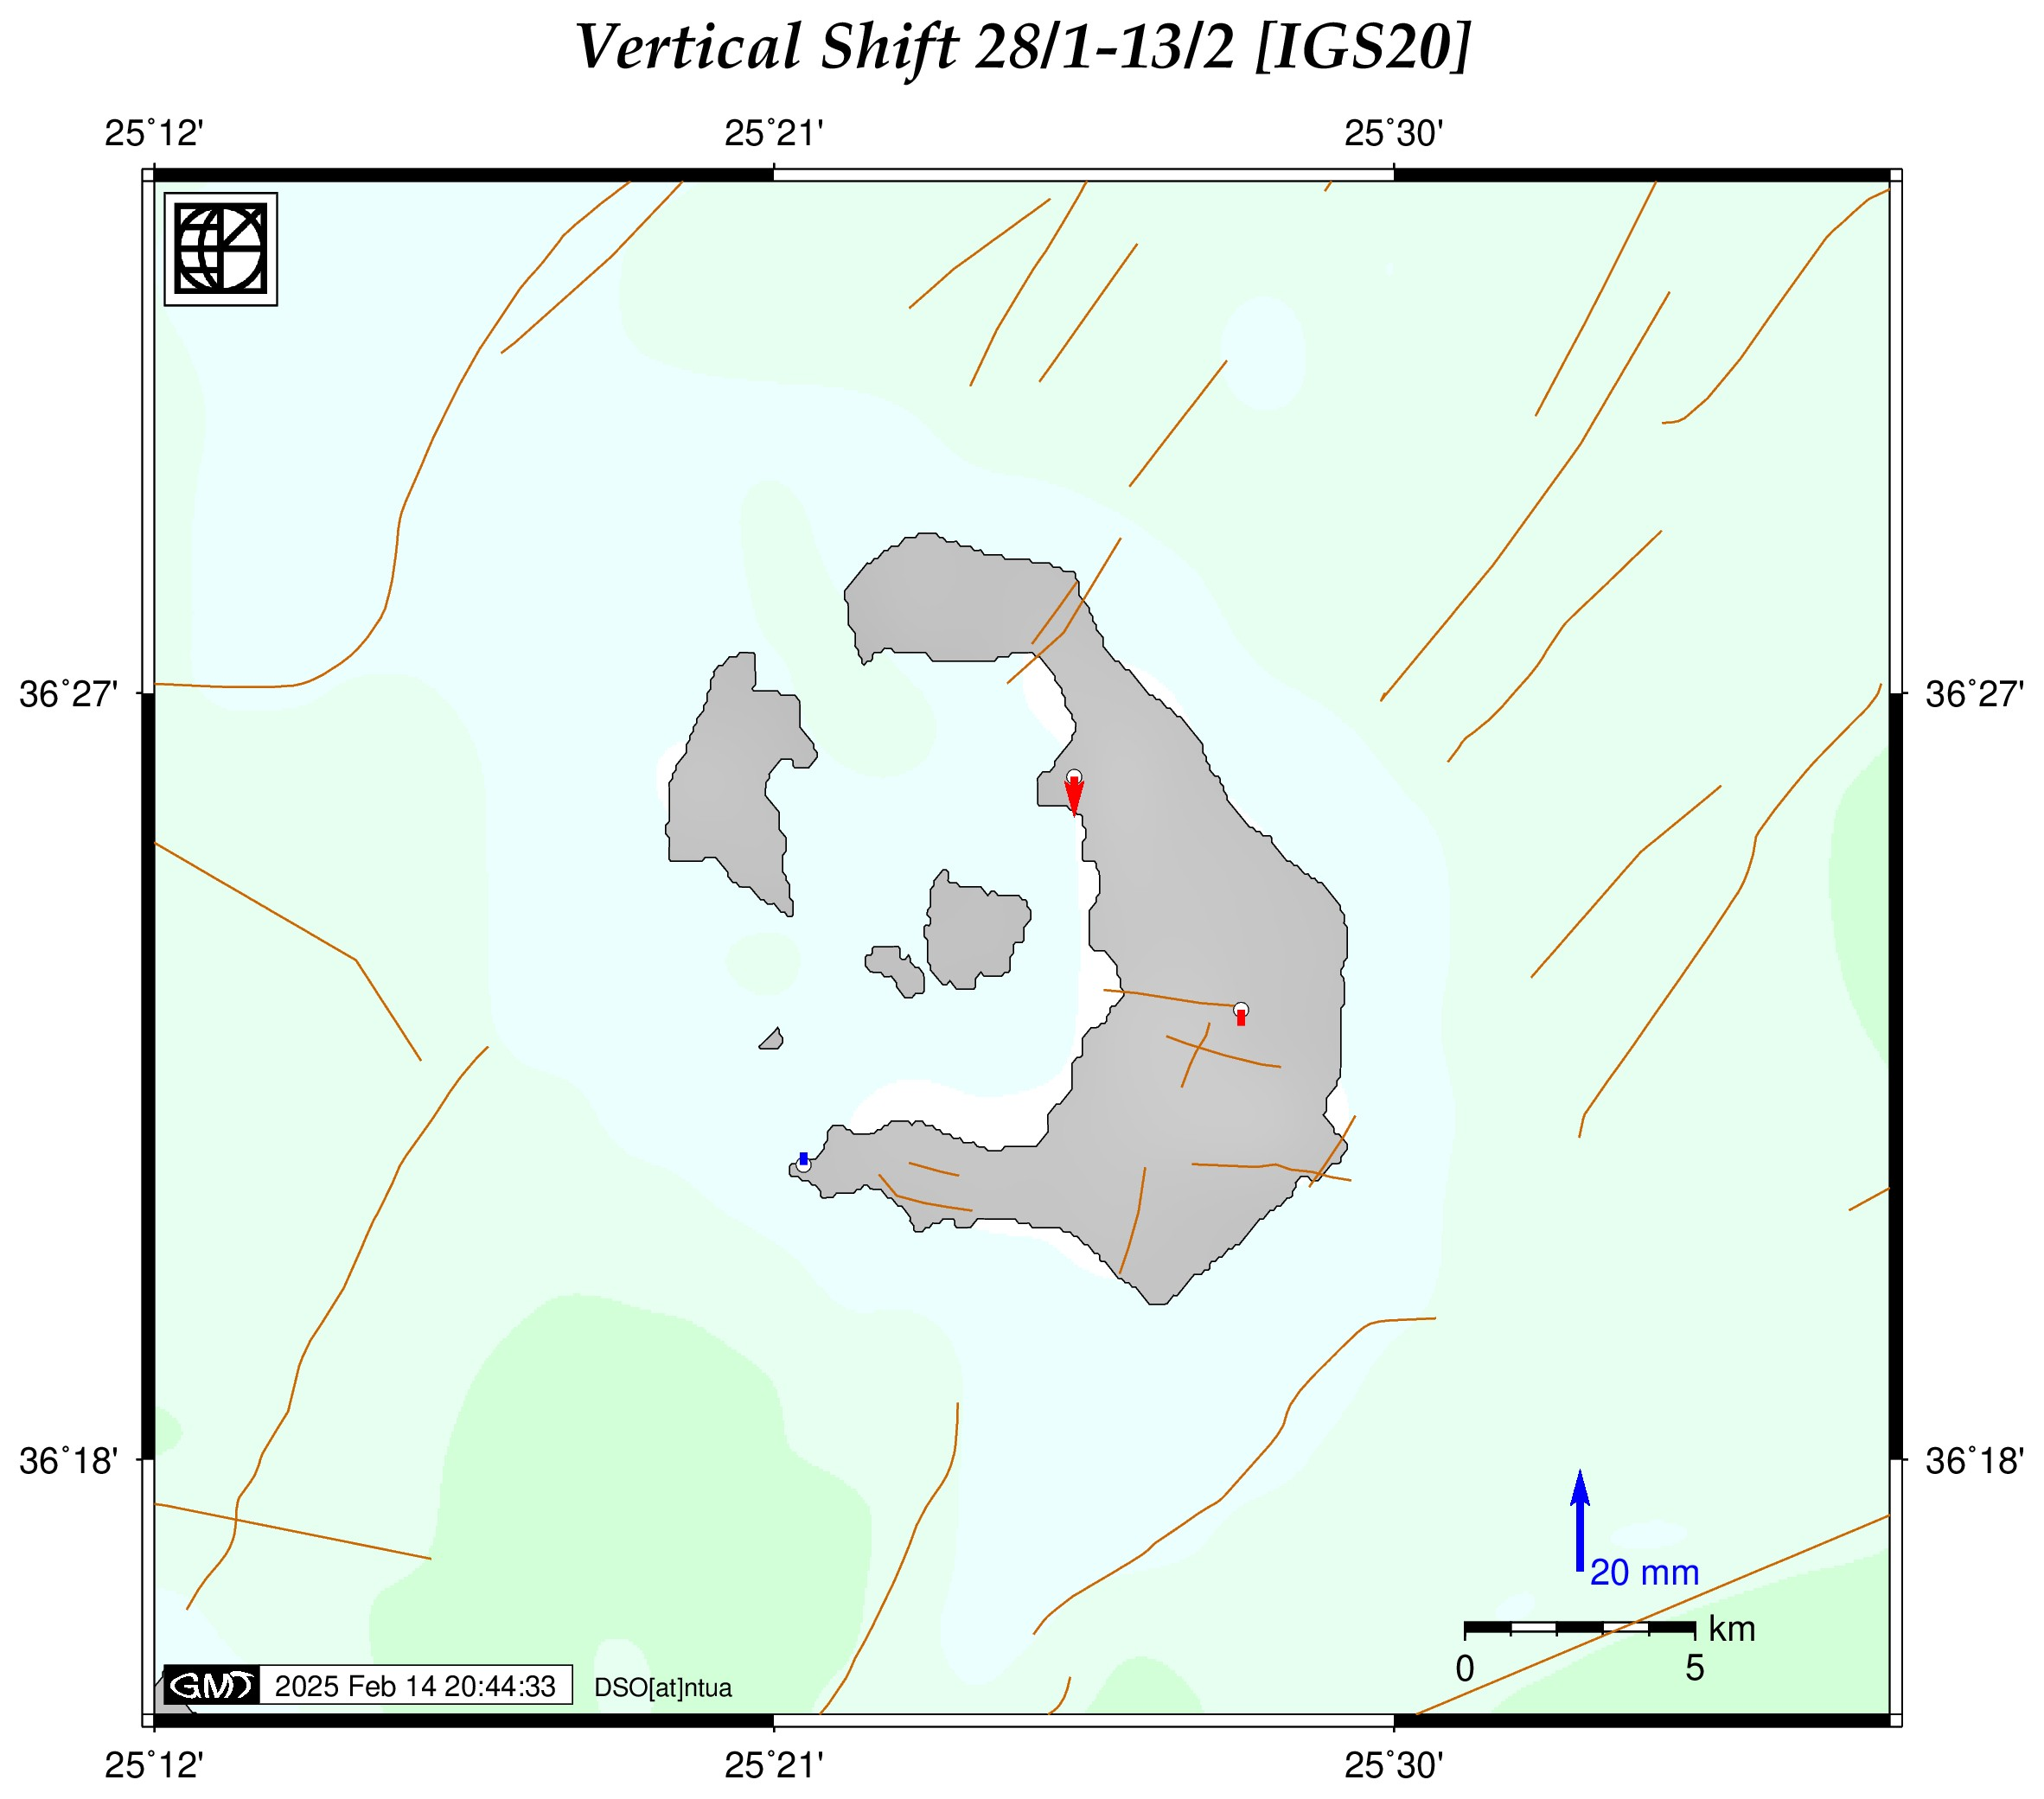
\includegraphics[width=.97\textwidth]{sant_2501_vver.jpg}
      \end{center}       
    \end{column}
  \end{columns}  

\end{frame}
\note{}

 % ------------------------------------------------------------------------------
\begin{frame}
  \frametitle{Station displacements 2025 28/1 - 25/2 }
  \framesubtitle{}
  \label{}
  \vskip-.5cm
  \begin{columns}[T]
    \begin{column}{.5\textwidth}
      \begin{center}
        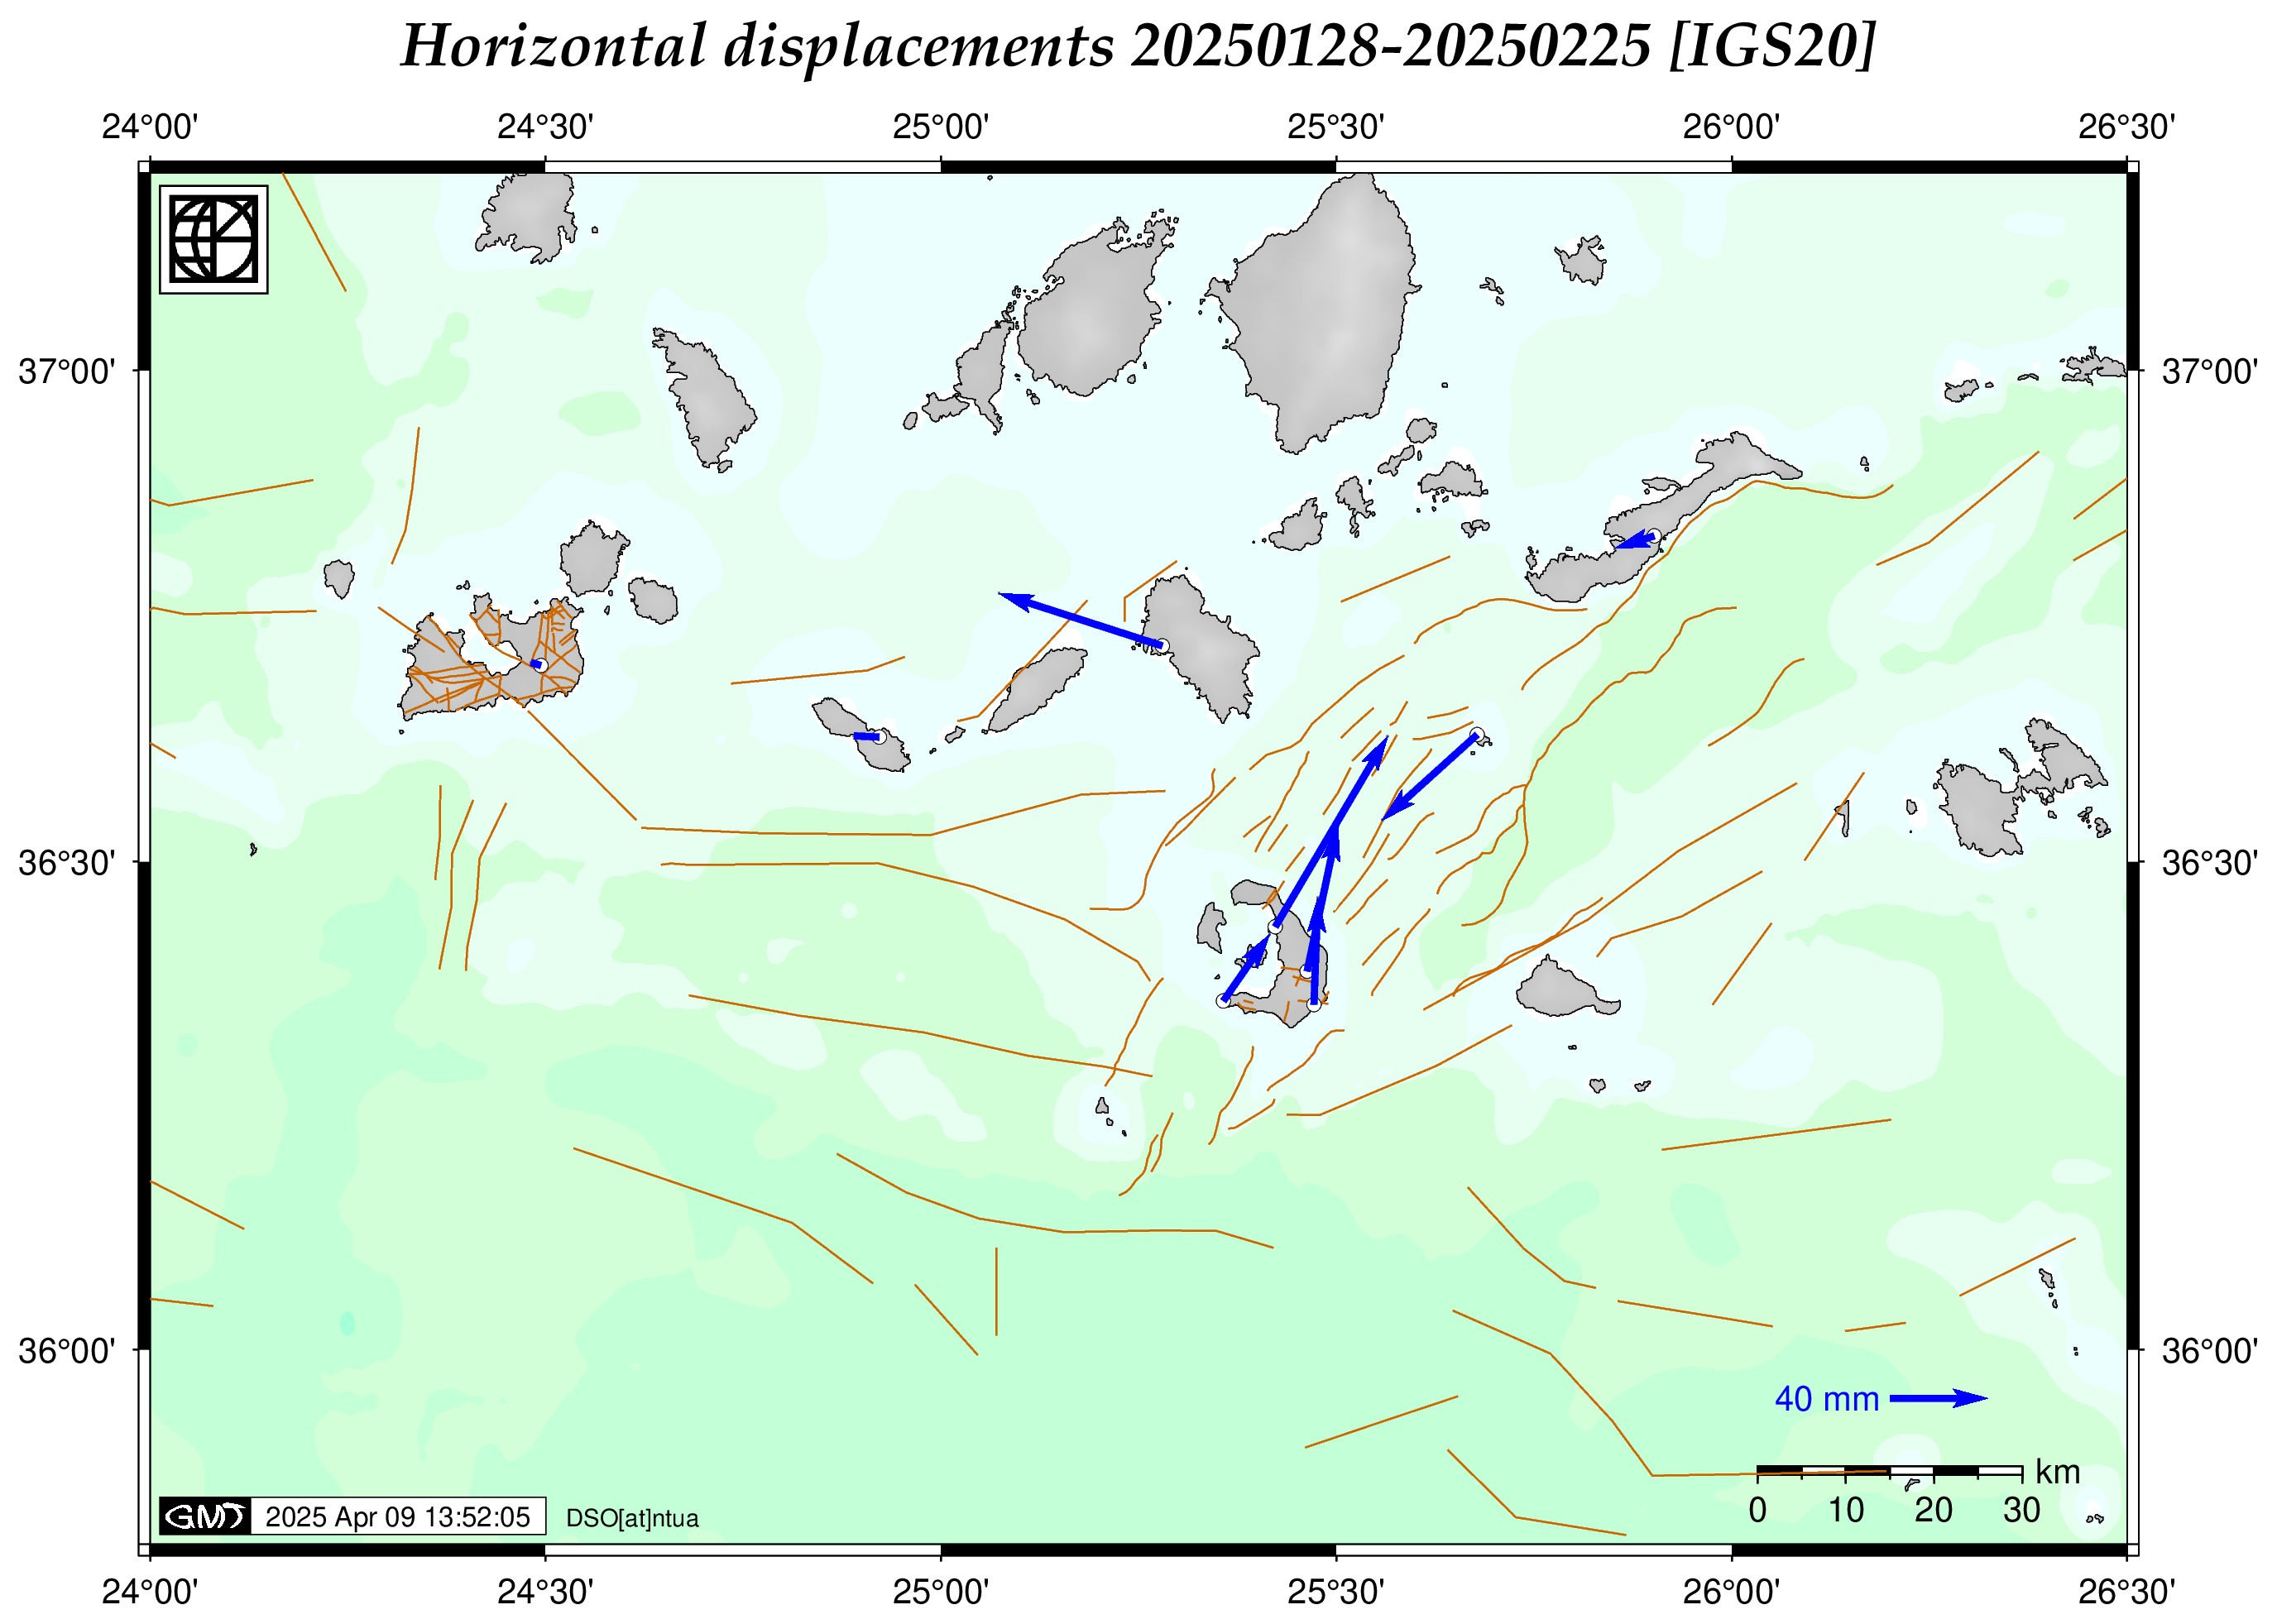
\includegraphics[width=.97\textwidth]{gnss_20250128_20250225_vhor.jpg}
      \end{center}  
    \end{column}
    \begin{column}{.5\textwidth}
      \begin{center}
        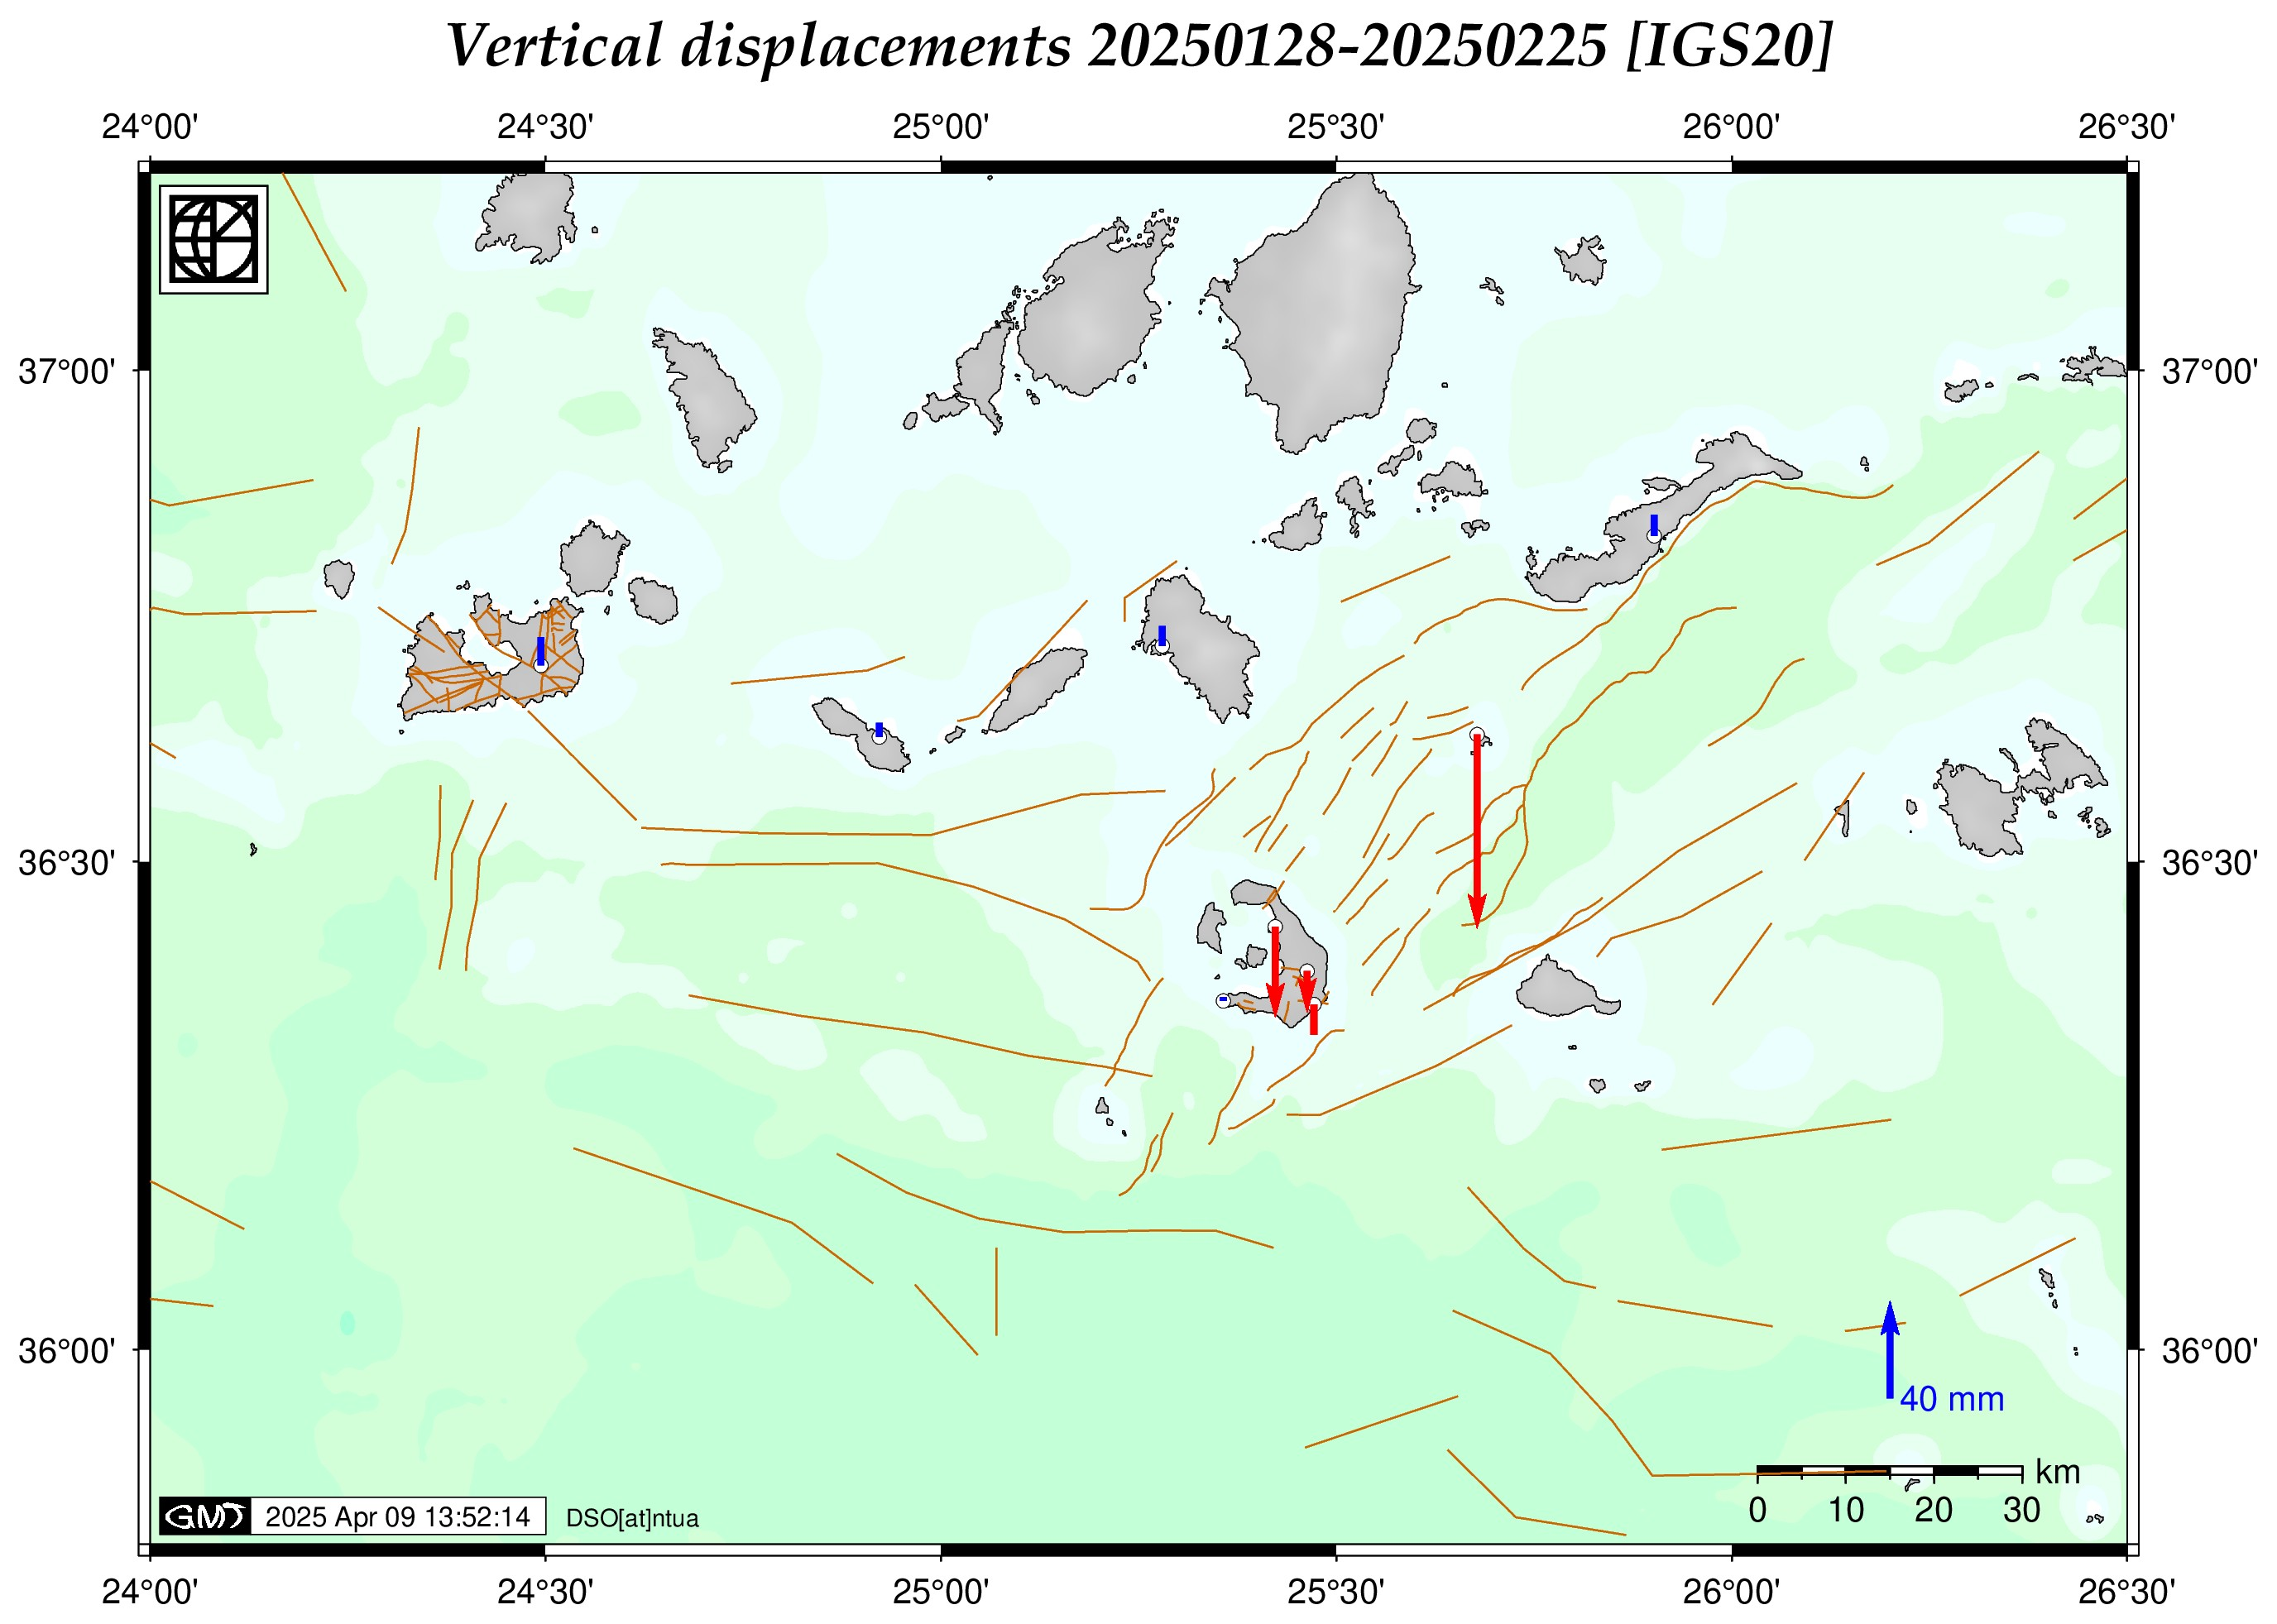
\includegraphics[width=.97\textwidth]{gnss_20250128_20250225_vver.jpg}
      \end{center}       
    \end{column}
  \end{columns}  

\end{frame}
\note{}

 % ------------------------------------------------------------------------------
\begin{frame}
  \frametitle{Relative distances (3D)}
  \framesubtitle{Santorini (048Α) - Amorgos (047Α) - Ios (049Α) - Anydros (ANYD)}
  \label{}
  \vskip-.8cm
  \begin{columns}[T]
    \begin{column}{.5\textwidth}
      \begin{center}
%      {\scriptsize 047A (Αμοργός)}
        
\includegraphics[width=.8\textwidth]{distvar_048a_047a.png}\\
        
\includegraphics[width=.8\textwidth]{distvar_048a_049a.png}
      \end{center}  
    \end{column}
    \begin{column}{.5\textwidth}
      \begin{center}
%       {\scriptsize 049A (Ίος)}
        
\includegraphics[width=.8\textwidth]{distvar_047a_049a.png}\\
        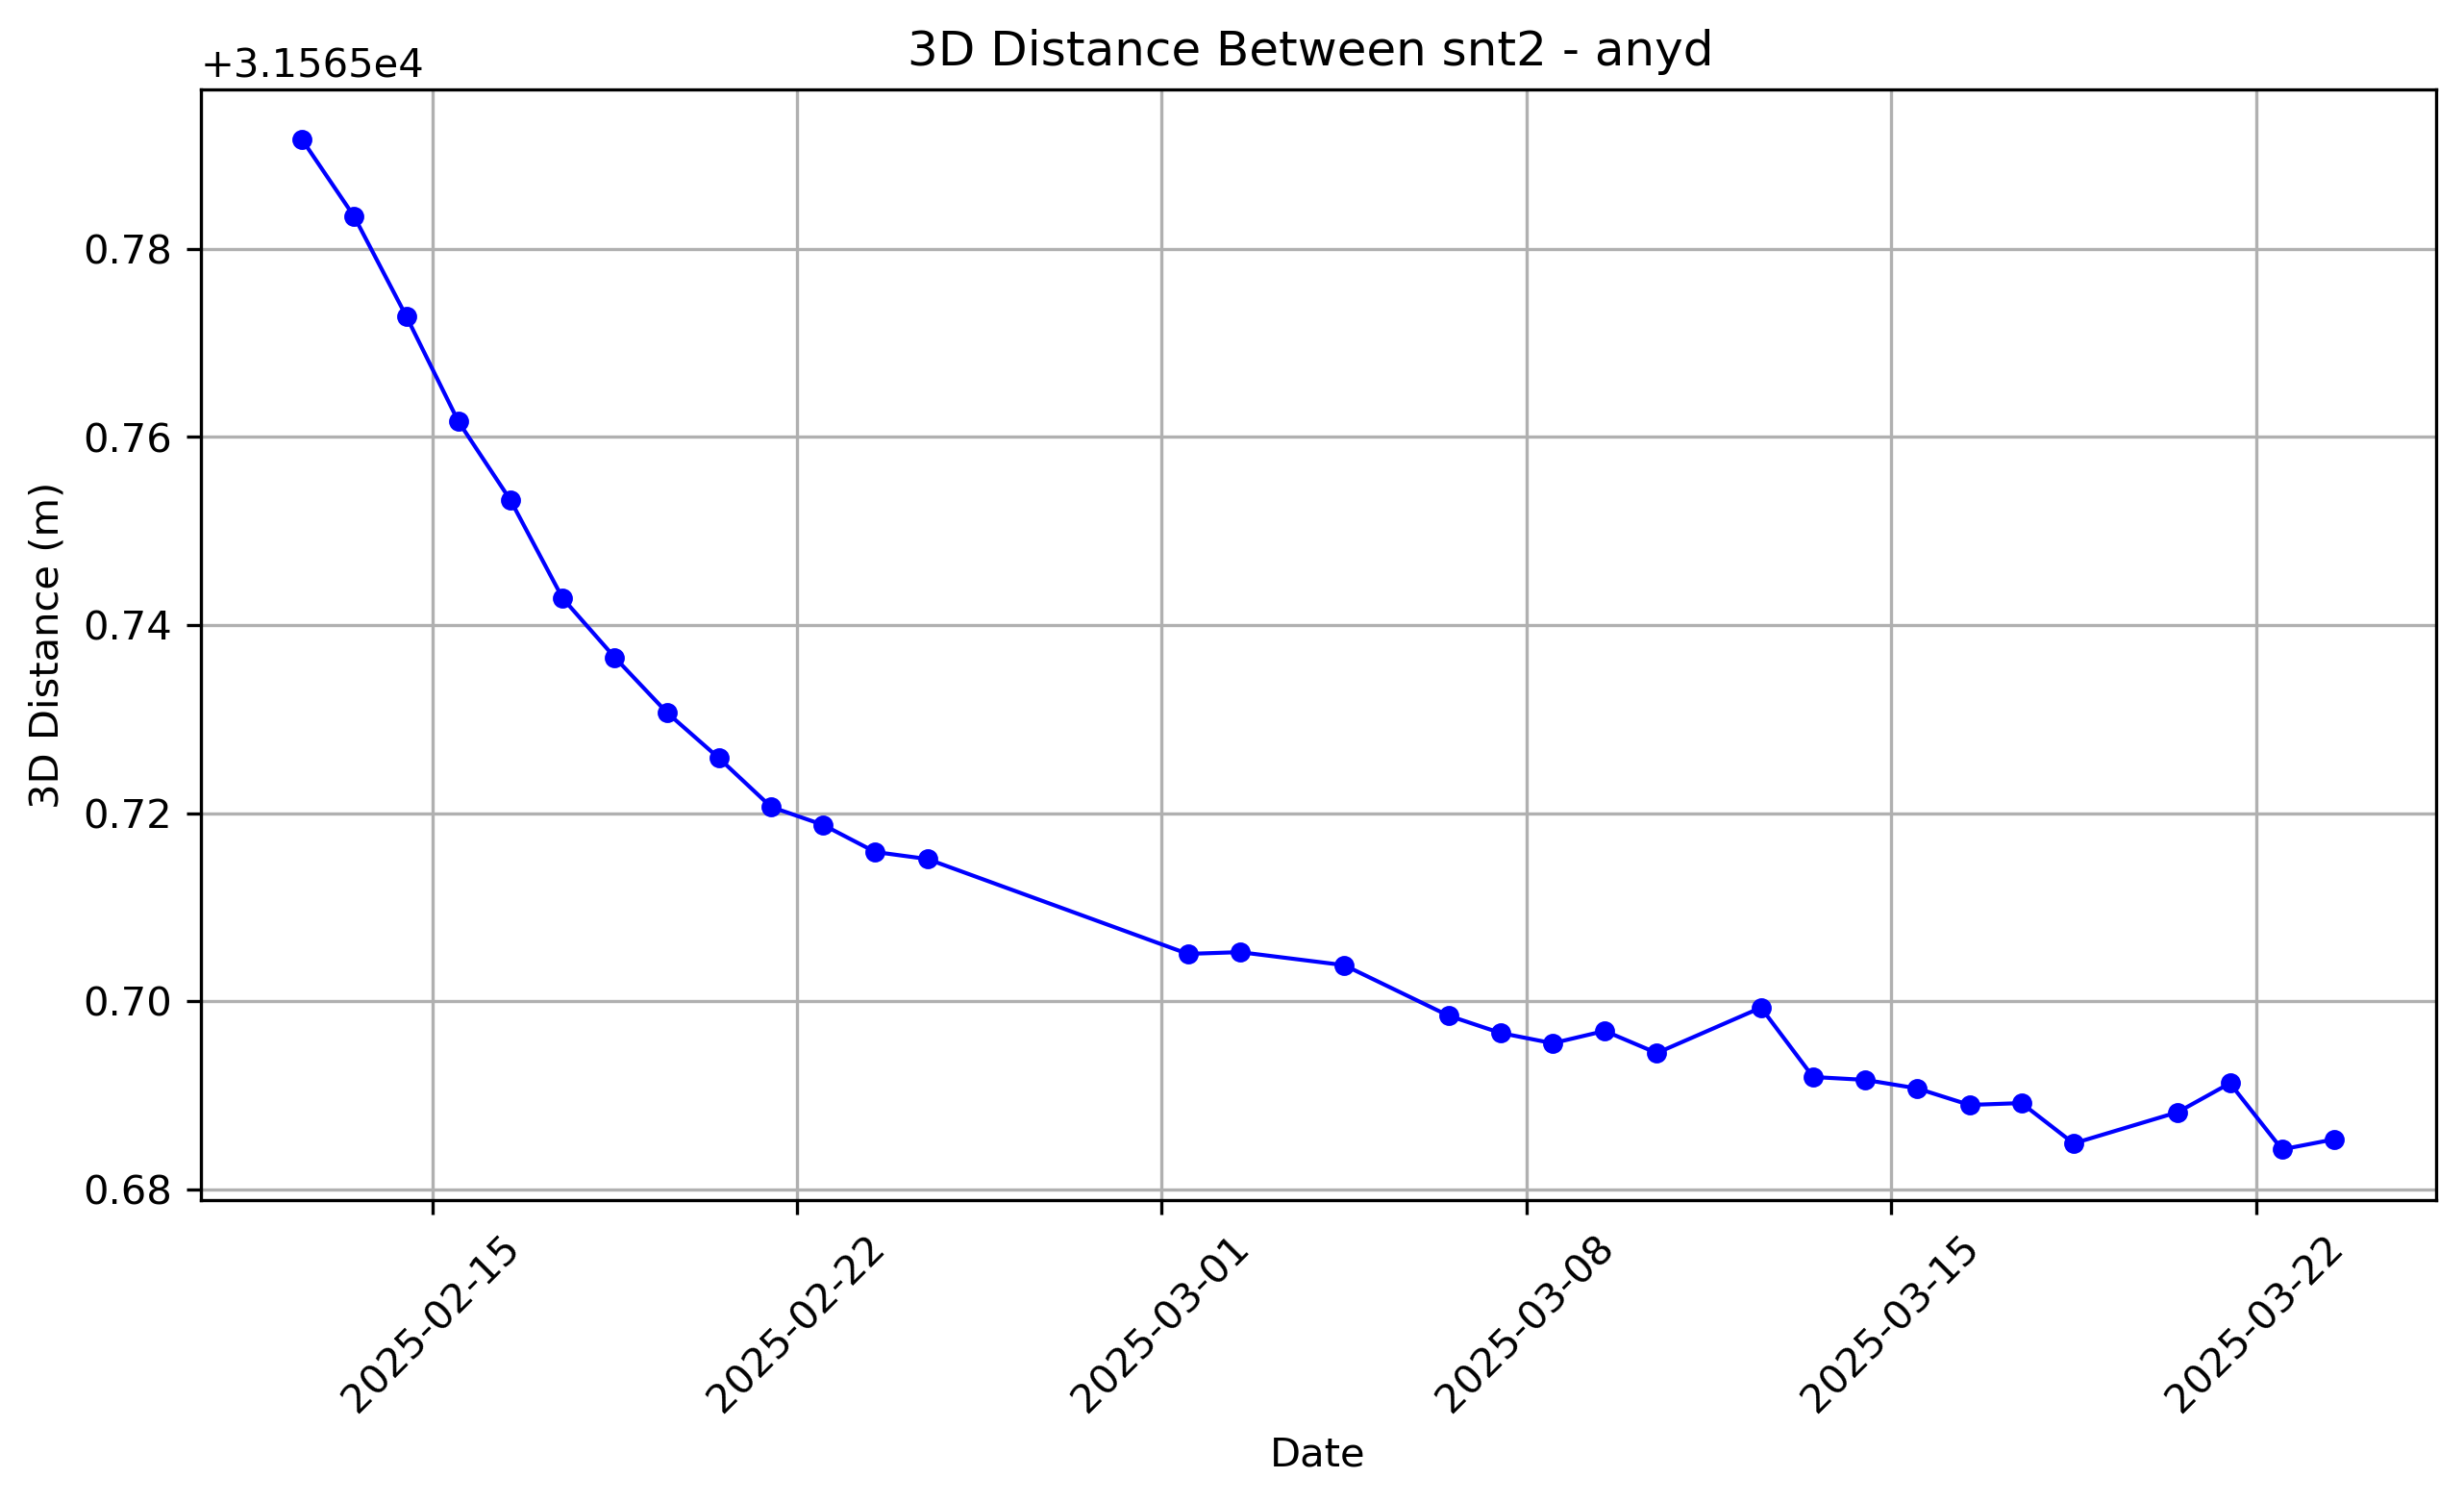
\includegraphics[width=.8\textwidth]{distvar_snt2_anyd.png}
      \end{center}       
    \end{column}
  \end{columns}  
  
\end{frame}
\note{}

 % ------------------------------------------------------------------------------
\begin{frame}
  \frametitle{High rate data analysis (1Hz)}
  \framesubtitle{}
  \label{}
  \begin{columns}[T]
    \begin{column}{.5\textwidth}
      \begin{center}
         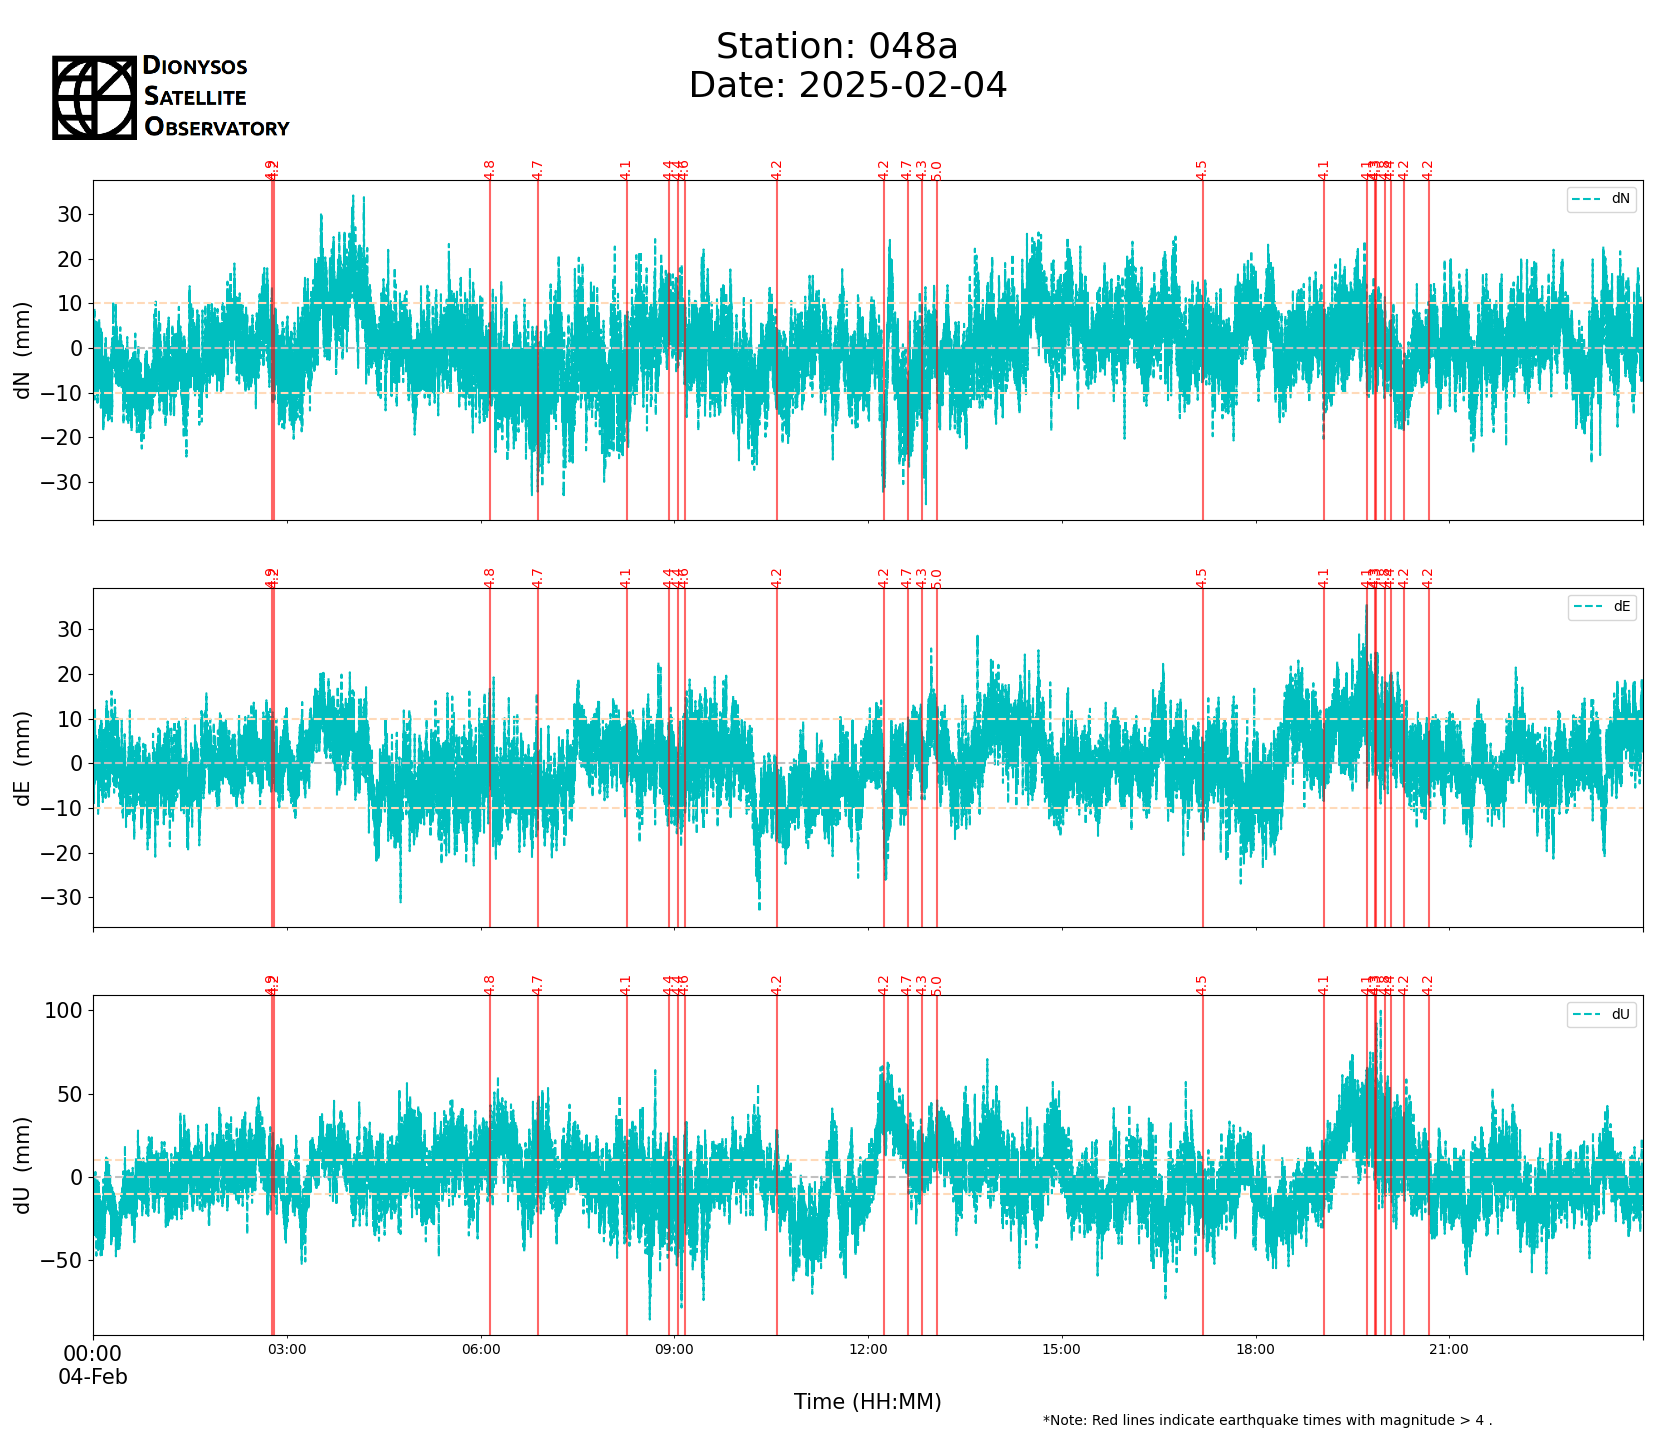
\includegraphics[width=.97\textwidth]{048a_25035.png}
       \end{center} 
    \end{column}
    \begin{column}{.5\textwidth}
      \begin{center}
        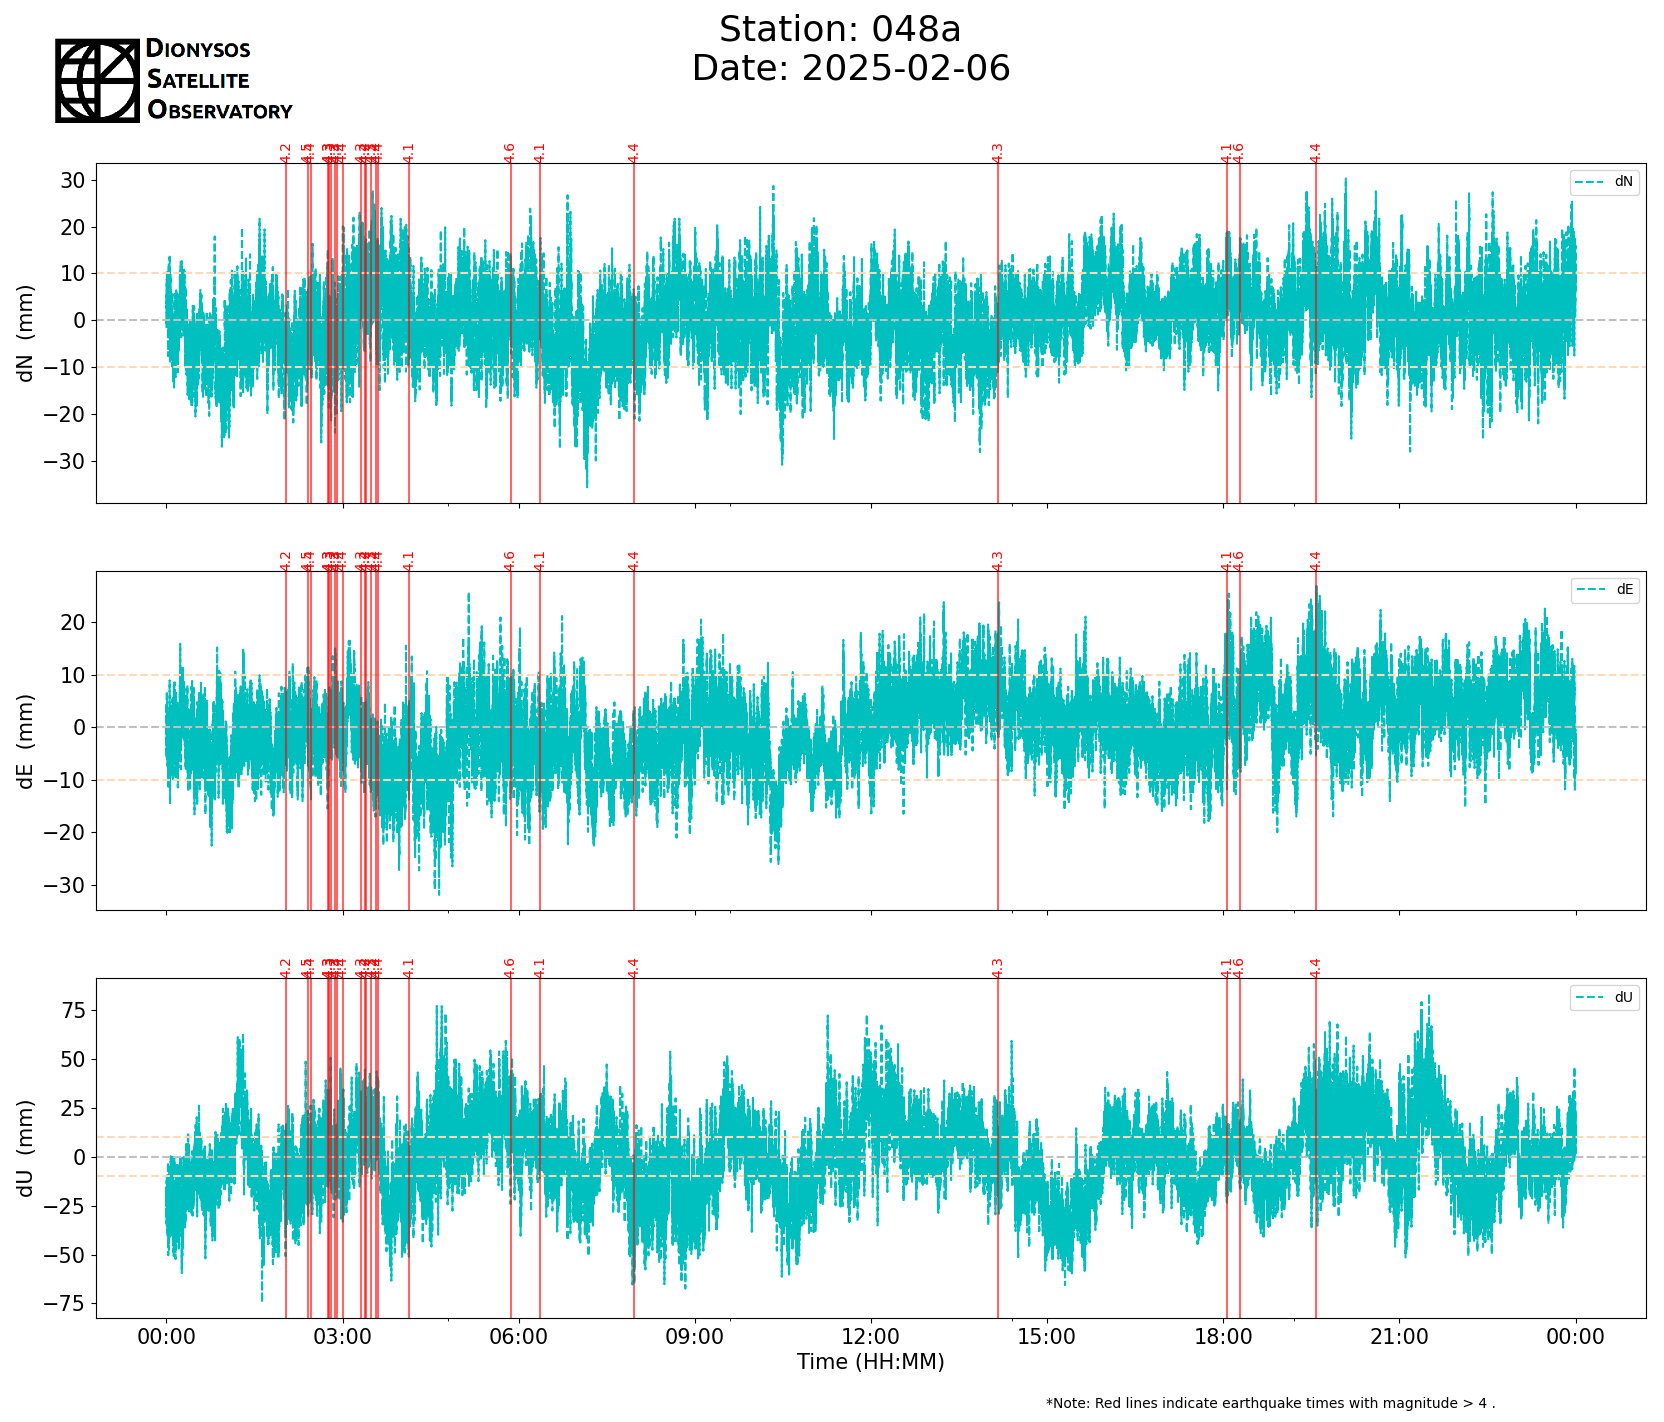
\includegraphics[width=.97\textwidth]{048a_25037.png}
      \end{center}
    \end{column}
  \end{columns}
\end{frame}
\note{}


 % ------------------------------------------------------------------------------
\begin{frame}
  \frametitle{DSO portal || Data \& Results dissemination}
  \framesubtitle{}
  \label{}
  \vskip-1.2cm
\begin{center}
  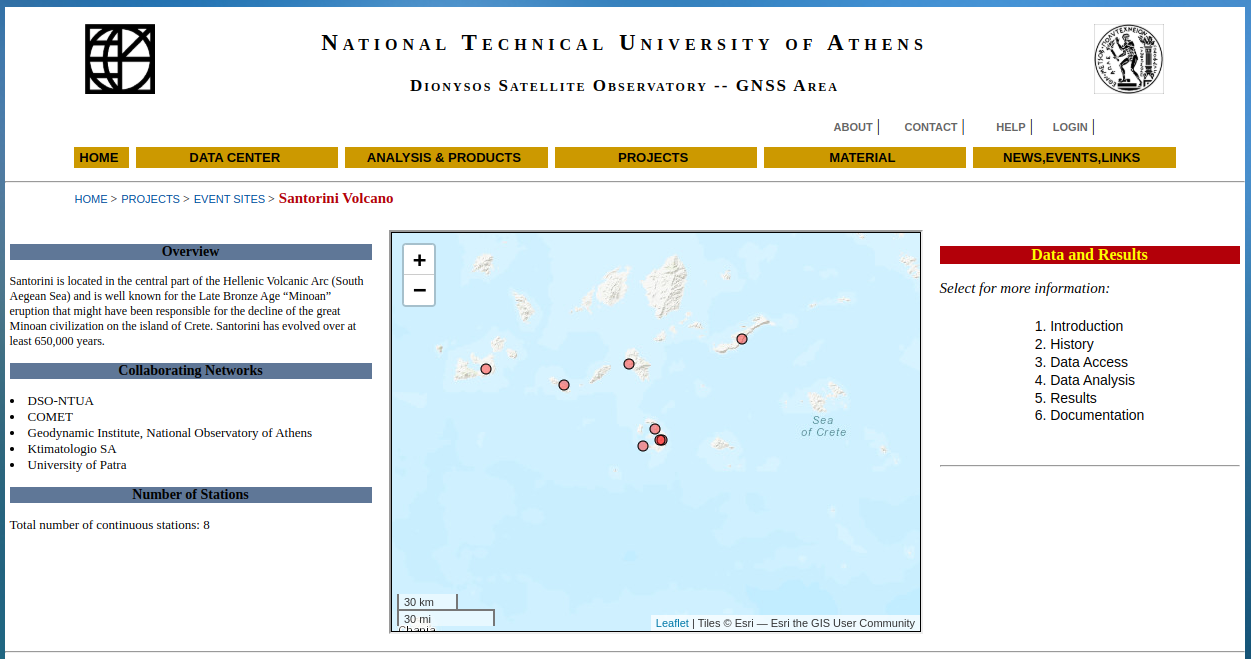
\includegraphics[width=.8\textwidth]{dsoportal_sant.png}
\end{center}
\url{http://dionysos.survey.ntua.gr/dsoportal/\_projects/supersites/santorini/}
\end{frame}
\note{}